\documentclass[12pt,reqno]{amsart}
\usepackage{graphicx}
\usepackage{amsfonts,amssymb,latexsym,amsmath}
\usepackage{tikz-cd}
\usepackage{mathrsfs}
\usepackage{enumerate}
\usetikzlibrary{arrows,calc,positioning,shadows,shapes}
\usepackage[cm]{fullpage}
\theoremstyle{plain}
\newtheorem*{theorem*}{Theorem}
%% this allows for theorems which are not automatically numbered
\newtheorem{defi}{Definition}
\newtheorem{theorem}{Theorem}
\newtheorem{lemma}{Lemma}
\newtheorem{obs}{Observation}
\newtheorem{exercise}{Exercise}
\newcommand{\heg}{\text{Heg}}
\newtheorem{rem}{Remark}
\newtheorem{disc}{Discussion}
\newtheorem{prop}{Proposition}
\newtheorem{coro}{Corollary}
\newtheorem{prob}{Problem}
\newtheorem{conv}{Convention}
\DeclareMathOperator{\spec}{Spec}
\DeclareMathOperator{\im}{im}
\DeclareMathOperator{\ann}{ann}
\DeclareMathOperator{\gal}{Gal}
\newtheorem{layout}{Layout}
\newcommand{\degg}{\textup{deg}}
\newtheorem{ex}{Example}
\usepackage{lineno}
\usepackage{hyperref}
\usepackage{xcolor}
\definecolor{winered}{rgb}{0.5,0,0}
\hypersetup{
    colorlinks=true,
    linkcolor=blue,
    filecolor=magenta,      
    urlcolor=winered,
}
%% The above lines are for formatting.  In general, you will not want to change these.
%%Commands to make life easier
\newcommand{\RR}{\mathbf R}
\newcommand{\aff}{\mathbb A}
\newcommand{\ff}{\mathbb F}
\newcommand{\cccC}{\mathbf C}
\newcommand{\oo}{\mathcal{O}}
\newcommand{\ZZ}{\mathbf Z}
\newcommand{\pring}{k[x_1, \ldots , x_n]}
\newcommand{\polyring}{[x_1, \ldots , x_n]}
\newcommand{\poly}{\sum_{\alpha} a_{\alpha} x^{\alpha}} 
\newcommand{\ZZn}[1]{\ZZ/{#1}\ZZ}
\newcommand{\QQ}{\mathbf Q}
\newcommand{\rr}{\mathbb R}
\newcommand{\cc}{\mathbb C}
\newcommand{\nn}{\mathbb N}
\newcommand{\zz}{\mathbb Z}
\newcommand{\cat}{\mathbf{C}}
\newcommand{\ca}{\mathbf}
\newcommand{\zzn}[1]{\zz/{#1}\zz}
\newcommand{\qq}{\mathbb Q}
\newcommand{\calM}{\mathcal M}
\newcommand{\latex}{\LaTeX}
\newcommand{\V}{\mathbf V}
\newcommand{\tex}{\TeX}
\newcommand{\sm}{\setminus} 
\newcommand{\dom}{\text{Dom}}
\DeclareMathOperator{\GL}{GL}
\DeclareMathOperator{\Hom}{Hom}
\newcommand{\sym}{\text{Sym}}
\newcommand{\ran}{\text{Ran}}
\newcommand{\pp}{\prime}
\newcommand{\gap}{\; \; \;}
\newcommand{\Mod}[1]{\ (\mathrm{mod}\ #1)}
\frenchspacing
\usepackage[shortlabels]{enumitem}
\usepackage{mdframed}
\usepackage{lipsum}
\def\boxitem#1{\setbox0=\vbox{#1}{\centering\makebox[0pt]{%
  \fboxrule=.5pt\color{black}\fbox{\hspace{\leftmargini}\color{black}\box0}}\par}}

\newcommand{\idealp}{\mathfrak{p}}
\newcommand{\rmod}{\textit{R}-\textbf{Mod}}
\newcommand{\idealP}{\mathfrak{P}}
\newcommand{\ideala}{\mathfrak{a}}
\newcommand{\idealb}{\mathfrak{b}}
\newcommand{\idealA}{\mathfrak{A}}
\newcommand{\idealB}{\mathfrak{B}}
\newcommand{\idealF}{\mathfrak{F}}
\newcommand{\idealm}{\mathfrak{m}}
\newcommand{\s}{\mathcal{S}}
\newcommand{\ccc}{\mathfrak{C}}
\newcommand{\idealM}{\mathfrak{M}}

\title{Piecing together crumbs: Introduction to Some Higher Algebra Topics}
\author{Juan Serratos}
\begin{document}
\begin{abstract}
%Originally, this paper was meant to be an introduction to basic notions of the tensor product between modules and some closely related material (e.g., biadditive functions, the $\Hom_R (A, B)$ set between two $R$-modules $A$ and $B$,  the category $R$-$\mathbf{Mod}$, etc...), but in trying to fit with my amorphous interests,  and my enjoyment of writing notes to myself, I'm deciding to fit this as a survey of some graduate school topics, that is, the tools and important notions one would typically learn from doing a PhD in pure mathematics, or, to a lesser extent, a Masters. Note: this isn't meant to be a complete overview of said curriculum, but just some topics that I find particularly interesting that require a solid understanding of undergraduate pure mathematics; 
Originally, this paper was meant to be an introduction to basic notions of the tensor product between modules and some closely related material (e.g., biadditive functions, the $\Hom_R (A, B)$ set between two $R$-modules $A$ and $B$,  the category $R$-$\mathbf{Mod}$, etc...) — a lot of the early sections for module theory and the appendices were written when I was a first year —  but now I think this paper is best understood as a paper that gives you a quick ``What is this thing? And how does it work?" of common \textit{things} in higher algebra. 

Now, with that out of the way, the topics that I've taken particular interest to discuss are: module theory (that is, essentially linear algebra but taken over a ring $R$ rather than a field, say, $F$), rudimentary topology to grasp at the notions of sheaves, category theory,  (co)homology, homotopy theory, and $\infty$-categories — motivated by reading early segments of Jacob Lurie's \textit{Higher Topos Theory}.  (However, I hope to further revise this \textit{paper} to include some sort of introduction to $p$-adic Hodge theory and the work of Peter Scholze with his notion of \textit{perfectoid rings and spaces}, but that'll require me to explain/develop the machinery in algebraic and arithmetic geometry, so I don't know). 
\end{abstract}
\begin{figure}[h] % htbp stand for "here", "top", "bottom", "page"
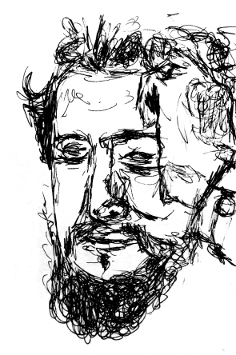
\includegraphics[scale=.2]{pic.png} 
\end{figure}
\maketitle
\tableofcontents
\newpage
\section{Motivation}

An introduction to learning about the tensor product and \textit{pure} tensors themselves are often times, in my experience, difficult to comprehend — or at least daunting. For example, if you're to pickup Eisenbud's \textit{Commutative Algebra with a View Toward Algebraic Geometry} you'll encounter the tensor product quickly enough and if you don't know already what it \textit{is} and \textit{does}, you might go the appendix and try to comprehend the definition. 
\begin{defi}[Eisenbud] Let $M$ and $N$ be $R$-modules. The \textbf{tensor product} of $M$ and $N$ over $R$, written $M \otimes_R N$, is the $R$-module generated by symbols $m \otimes n$ for $m \in M$ and $n \in N$, with relations 
\begin{align*}
rm \otimes n &= m \otimes rn \\
(m + m^{\prime}) \otimes n &= m \otimes n + m^{\prime} \otimes n  \\
m \otimes (n + n^{\prime}) &= m \otimes n + m \otimes n^{\prime}.
\end{align*}
\end{defi} 

Eisenbud then states, immediately, that ``these relations say precisely that the natural map 
\\ $b \colon M \times N \to M \otimes_R N$ taking $(m, n)$ to $m \otimes n$ is \textbf{bilinear}." Now, as for me, I immediately thought ``What the fuck is bilinear?" I had taken a computationally focused linear algebra course in high school so the theoretical ideas didn't really stick, and so it took some formal linear algebra enlightenment to further understand what Eisenbud was talking about. Really what this exposition is all about is an introduction, or refreshment, of the formal linear algebra ideas that mathematicians seems to always bring up — you simply cannot avoid linear algebra in any of the natural science, nor mathematics (this is a topic that is milked so much).  

Now, another aspect of this exposition that may be useful is the categorical foundations that I may get into since they're as well used so often in say commutative algebra, homological algebra, algebraic geometry, K-theory, algebraic topology, and by god this list can likely stretch so far out. And well you probably suspected it, they're also integral in understanding different perspectives (or you may argue the main perspective) of the tensor product. For example, as Eisenbud continues talking about the tensor product in his appendix (Appendix A2. Multilinear Algebra): ``It is elementary that a bilinear map $M \times N \to P$ is the same as a homomorphism $M \to \Hom_R (N, P)$, so we may rewrite the natural isomorphism above as a natural isomorphism 
$$ \Hom_R (M \otimes_R N, P) \cong \Hom_R (M, \Hom_R (N, P)).$$
In categorical language this says that the functor $- \otimes_R N$ is the left adjoint functor of the functor $\Hom_R (N,  -)$. "

Although I've mentioned the case of approaching Eisenbud's tensor product definition, there are some other examples that I think are fruitful in mentioning since I'll be trying to really, in a way, comprehend them (myself included) in later sections. 


One that comes to mind is provided in Joseph Rotman's \textit{An Introduction to Homological Algebra}. This definition, however, requires more machinery; first we need to describe what we mean by bilinear, and thus we also need to know what biadditive is.  This is all in having the idea of describing the tensor product as a biadditive function between modules, or in the \textit{special case}, between vector spaces. 
\begin{defi}[Rotman] Let $R$ be a ring , let $A_R$ be a right $R$-module, let $_R B$ be a left $R$-module, and let $G$ be an (additive) abelian group. A function $f \colon A \times B \to G$ is called $R$-\textbf{additive} if, for all $a, a^{\prime} \in A, b, b^{\prime} \in B$, and $r \in R$, we have 
\begin{align*}
f(a+a^{\prime}, b) &= f(a, b) + f(a^{\prime}, b), \\
f(a, b+b^{\prime}) &= f(a, b)+ f(a, b^{\prime}), \\
f(ar, b) &= f(a, rb).
\end{align*}

If $R$ is \textit{commutative} and $A$, $B$, and $M$ are $R$-modules, then a function $f \colon A \times B \to M$ is called $R$-\textbf{bilinear} if $f$ is $R$-biadditive and also
$$f (ar, b) = f(a, rb) = r f(a, b)$$
$[rf(a, b)$ makes sense here because $f(a, b)$ now lies in the $R$-module $M]$. 
\end{defi} 

A clear example, that Rotman provides,  is that if we have a ring $R$, then we will get, naturally, that its multiplication $\varphi \colon R \times R \to R$ is $R$-additive — as Rotman says, ``the first two axioms are the right and left distributive laws, while the third axiom is associativity." You can check these easily on your own.  Now, since we didn't assume $R$ to be commutative, we can then suppose that it is and then we'll get that $\varphi$ is bilinear since $\varphi \colon R \times R \to R$ is biadditive and $\varphi (ar, b) = (ar)b= a(rb) = \varphi (a, rb) = r(ab) = r \varphi (a, b)$ also holds. 

The purpose of describing all this machinery is to simply explain the tensor product as a sort of conversion process between biadditive functions and linear functions.
\begin{rem}[Rotman]The tensor product converts biadditive functions into linear ones. 
\end{rem} 
\begin{defi}[Rotman] Given a ring $R$ and modules $A_R$ and $_R B$, then their \textbf{tensor product}  is an abelian group $A \otimes_R B$ and an $R$-biadditive function
$$ h \colon A \times B \to A \otimes_R B$$ such that, for every abelian group $G$ and every $R$-biadditive $f \colon A \times B \to G$, there exists a unique $\zz$-homomorphism $\tilde{f} \colon A \otimes_R B \to G$ making the following diagram commute. 
$$\begin{tikzcd}
A \times B \arrow[rrrr, "h"] \arrow[rrdd, "f"'] &  &   &  & A \otimes_R B \arrow[lldd, "\tilde{f}", dashed] \\
                                       &  &   &  &                             \\
                                       &  & G &  &                            
\end{tikzcd}$$
\end{defi} 

A $\zz$-homomorphism is an abelian homomorphism. Moreover, if you can't recall immediately what a linear function is, as it's important to know for Remark 1:
\begin{defi} A \textbf{linear function} is a mapping $\lambda \colon A \to M$ between $R$-modules $A$ and $M$ such that it satisfies the properties
\begin{align*}
\lambda (a+b) &= \lambda (a) + \lambda (b), \\
\lambda (\alpha b) &= \alpha \lambda (b),
\end{align*}
for all $a, b \in A$ and $\alpha \in R$.
\end{defi} 
Rotman's definition of the tensor product gave us a look at how categorical methods (specifically, diagram chasing) are going to be a great tool. For example, the following proposition uses categorical methods in its proof:
\begin{prop} If $A \otimes_R B$ and $\mathfrak{T}$ are tensor products of $A$ and $B$ ($R$-modules) over $R$, then $A \otimes_R B \cong \mathfrak{T}$.
\end{prop} 
\begin{proof} Suppose that $\partial \colon A \times B \to \mathfrak{T}$ is an $R$-biadditive function such that, for every abelian group $G$ and every $R$-biadditive $f \colon A \times B \to G$, there exists a a unique $\zz$-homomorphism $\tilde{f} \colon \mathfrak{T} \to G$ such that $f$ commutes via $\tilde{f} \partial$, i.e., $\tilde{f} \partial = f$.

However, rather than going through nearly the same process of defining all the same assumptions for $A \otimes_R B$ being a tensor product of $R$-modules of $A$ and $B$, we can just justify all our assumptions with the fact that the following diagram 

$$\begin{tikzcd}
\mathfrak{T} \arrow[rrrrdd, "\tilde{f}"', dotted] &  &  &  & A\times B \arrow[rrrr, "\eta"] \arrow[llll, "\partial"'] \arrow[dd, "h"', shift right] \arrow[dd, "f", shift left] &  &  &  & A \otimes_R B \arrow[lllldd, "\tilde{h}", dotted] \\
                               &  &  &  &                                                                                                  &  &  &  &                               \\
                               &  &  &  & G                                                                                                &  &  &  &                              
\end{tikzcd}$$ 
commutes with two unique $\zz$-homomorphisms $\tilde{f}$ and $\tilde{h}$, and that $\eta \colon A \times B \to A \otimes_R B$ is an $R$-biadditive function with the obvious assumption that for every $R$-biadditve $f \colon A \times B \to G$, it commutes with $\tilde{h} \colon A \otimes_R B \to G$. 

Now setting $ A \otimes_R B$ = $G$ and $f = h$, since $A \otimes_R B$ is an abelian group so we can since we made no assumptions about $G$, we get, trivially, that there's a unique $\zz$-homomorphism $\tilde{f} \colon \mathfrak{T} \to A \otimes_R B = G$; thus, $ f = \tilde{f} \partial$.  Furthermore, we do something very similar with the fact that $A \otimes_R B$ is a tensor product: we can set $G = \mathfrak{T}$ and there will be, with the usual assumptions made about the tensor product above,  a unique $\zz$-homomorphism $\tilde{h} \colon A \otimes_R B \to \mathfrak{T}$ that commutes via $h = \tilde{h} \eta$.  (If you didn't catch the assumptions made, it follows formally as: Suppose $\eta \colon A \times B \to A \otimes_R B $ is an $R$-biadditive function such that, for every abelian group $G$ and every $R$-biadditive $h \colon A \times B \to G$, there exists a unique $\zz$-homomorphism $\tilde{h} \colon \mathfrak{T} \to G$.) 

Conisder the following diagram
$$\begin{tikzcd}
                                                            &  &  &  & A \otimes_R B \arrow[dd, "\tilde{f}", dotted] \arrow[dddd, "1_{A \otimes_R B}", bend left, shift left=2] \\
                                                            &  &  &  &                                                                      \\
A \times B \arrow[rrrr, "\partial"] \arrow[rrrruu, "\eta"] \arrow[rrrrdd, "\eta"] &  &  &  & \mathfrak{T} \arrow[dd, "\tilde{h}", dotted]                                            \\
                                                            &  &  &  &                                                                      \\
                                                            &  &  &  & A \otimes_R B                                                                   
\end{tikzcd}$$ 
The diagram commutes since we have that $\tilde{f} \colon A \otimes_R B \to \mathfrak{T}$ and $\tilde{h} \colon \mathfrak{T} \to A \otimes_R B$ both exist due to our assumptions. Moreover, we see that that the big triangle commutes by $\eta = \tilde{h} \tilde{f}$ but also by $1_{A \otimes_R B}$, and thus $1_{A \otimes_R B} = \tilde{h} \tilde{f}$. As an exercise, you should prove that the other part of the isomorphism holds true, i.e., $1_{\mathfrak{T}} = \tilde{f} \tilde{h}$. However, I'll also sort of do it here: In the diagram defining $A \otimes_R B$, we set $\mathfrak{T} = G$ and get that the following diagram 
$$\begin{tikzcd}
                                                            &  &  &  & \mathfrak{T} \arrow[dd, "\tilde{f}", dotted] \arrow[dddd, "1_{\mathfrak{T}}", bend left, shift left=2] \\
                                                            &  &  &  &                                                                      \\
A \times B \arrow[rrrr, "\eta"] \arrow[rrrruu, "\partial"] \arrow[rrrrdd, "\partial"] &  &  &  & A \otimes_R B \arrow[dd, "\tilde{h}", dotted]                                            \\
                                                            &  &  &  &                                                                      \\
                                                            &  &  &  & \mathfrak{T}
\end{tikzcd}$$ commutes with $1_{\mathfrak{T}} = \tilde{f} \tilde{h}$. Therefore, $A \otimes_R B \cong \mathfrak{T}$. (\textbf{Revise Proof:} fix definitions of $\tilde{f}$ and $\tilde{h}$.)
\end{proof} 
\newpage 
\section{Module Theory}
\subsection{Definition and Examples}
To establish some common notation, and provide a general refresher, we'll go through an introduction to the ideas of module theory. If this topic is unknown to you, it's a \textit{weaker} theory of vector spaces: a vector space takes its scalars from a field (e.g., $\rr$, $\cc$, $\qq$, etc...), while a module takes its scalars from a ring (e.g., $\zz$, $\zz [i]$, etc...).

Some lore from the famous \textit{Abstract Algebra} by Dummit $\&$ Foote: ``The use of modules was pioneered by one of the most prominent mathematicians of the first part of this century, Emmy Noether, who led the way in demonstrating the power and elegance of this structure. We shall see that vector spaces are just special types of modules which arise when the underlying ring is a field. If $R$ is a ring, the definition of an $R$-module $M$ is closely analogous to the definition of a group action where $R$ plays the role of the group and $M$ the role of the set. The additional axioms for a module require that $M$ itself have more structure (namely that M be an abelian group). Modules are the `representation objects' forrings, i.e., they are, by definition, algebraic objects on which rings act. As the theory develops it will become apparent how the structure of the ring $R$ (in particular, the structure and wealth of its ideals) is reflected by the structure of its modules and vice versa in the same way that the structure of the collection of normal subgroups of a group was reflected by its permutation representations."

\begin{defi} Let $R$ be a ring. By an $R$-\textbf{module} $M$, we mean an additive abelian group $M$ together with a map $R \times M \to M$, $(a, x) \mapsto ax$, called \textbf{scalar multiplication}, satisfying the following conditions for all $a, b \in R$, and $x, y \in M$: 
\begin{align*}
a(x+y) & = ax + ay,  \\
(a+b) x &= ax + bx, \\
a(bx) &= (ab)x, \\
1x &= x.
\end{align*}
If $R$ is not necessarily commutative then the above conditions define a \textbf{left} $R$-\textbf{module}; commonly denoted as $_R M$.  For a \textbf{right} $R$-\textbf{module}, the third condition $(xb)a = x(ba)$ defines the right $R$-module, which is commonly denoted $M_R$. Elements in a $R$-module $M$ are called \textbf{vectors} and elements in the underlying ring are called \textbf{scalars}. 
\end{defi} 

\begin{rem} We call the map $R \times M \to M$ an $R$-\textit{action}.
\end{rem} 


In this paper, we focus our discussion on commutative rings, and so the notions of right and left don't need to be specified since commutivity will provide that they coincide; that is, $a(bx) = (ab)x = (xb)a = x(ba)$.  However, there may be some remarks of some properties that also hold for modules where their ring of scalars are not necessarily commutative. 

Some examples of $R$-modules — if said without context, you should assume $R$ is a commutative ring with unity:
\begin{itemize}
\item A ring $R$ is an $R$-module over itself 
\end{itemize}

For an $R$-module $M$, properties of the following type are deduced easily from the above axioms: $a0 = 0 = 0x, (-1)x = -x, (-a)x = a(-x) = -(ax), (a-b)x=ax-bx, a(x-y)=ax-ay$, $a \left( \sum x_i \right) = \sum ax_i$, $\left( \sum a_i \right) x = \sum a_i x $, etc. Here $a,a_i, b \in R$, $x, x_i, y \in M$, and the symbol $0$ is used to denote the additive identity of both $R$ and $M$.
\begin{defi} Let $M$ be an $R$-module. A nonempty subset $N$ of $M$ is called a \textbf{submodule} (more precisely, an $R$-submodule) of $M$ if for any $a \in R$ and $x, y \in N$, we have $x+y \in N$ and $ax \in N$, that is, $N$ is itself an $R$-module.
\end{defi}


\begin{rem} Submodules of $M$ are therefore just subsets of $M$ which are themselves modules under the restricted operations. In particular, if $R = F$ is a field, submodules are the same as subspaces. Every $A$-module $M$ has the two submodules $M$ and $0$ (the latter is called the \textbf{trivial submodule}).
\end{rem}
\begin{prop} Suppose $R$ is a ring. Let $\{ M_i \}$ be a family of submodules of a module $M$. Then $\bigcap_i M_i$ is also a submodule of $M$
\end{prop}
\begin{proof} Clearly $\bigcap_i M_i$ is nonempty since $0$ is in every submodule. Let $x, y \in \bigcap_i M_i$. Then $x, y$ are contained in every submodule of $\{M_i \}$, and so let $x, y \in M_{\alpha}$ for some $M_{\alpha} \in \{M_i \}$. But then $x+y \in M_{\alpha}$ by mere definition of a submodule, and so $x+ y \in \bigcap_i M_i$. Moreover, let $a \in R$ and $x \in M_{\alpha}$. Then, once again, by definition, we have that $ax \in M_{\alpha}$, and so $ax \in \bigcap_i M_i$. Therefore $\bigcap_i M_i$ is a submodule of $M$. 
\end{proof}
\begin{ex}[$\zz$-modules] Let $R = \zz$, let $A$ be any abelian group (finite or infinite) and write the operation of $R$ as $+$. Make $R$ into a $\zz$-module as follows: for any $n \in \zz$ and $a \in R$ define 
\[ na = 
\begin{cases} 
a+a + \cdots + a \textup{ ($n$ times)} & \textup{if } n > 0\\
0 & \textup{if } n = 0 \\
-a-a-\cdots-a \textup{ ($-n$ times)} & \textup{if } n<0
\end{cases}
\]
(here $0$ is the identity of the additive group $A$). This definition of an action of the integers on $A$ makes $A$ into a $\zz$-module. 
\end{ex}
\begin{ex} Let $_RM$ be an $R$-module and let $M_1, M_2, \ldots, M_n$ be submodules of $_RM$.  Define \[ M_1 + M_2 + \cdots + M_n = \{x_1 + x_2 + \cdots + x_n \mid x_i \in M_i, i=1, 2, \ldots, n \} .\]

It is easy to see that $M_1 + M_2 + \cdots + M_n$ is a submodule of $_RM$, which is called the \textbf{sum} of $M_1 + M_2 + \cdots + M_n$.  More generally, let $\{M_i \mid i \in \Lambda \}$ be a family of submodules of $M$.  Define \[ \sum_i M_i =\{x_{i_1} + x_{i_2} + \cdots + x_{i_n} \mid x_{i_k} \in M_{i_k}, i_k \in \Lambda,  n \in \zz_{>0} \} .\] 

Then $\sum_{i \in \Lambda} M_i$ is a submodule of $M$, which is called the \textbf{sum} of $\{M_i \mid i \in \Lambda \}$
\end{ex}

Since ever ideal of $R$ is a submodule of $R$, the above sum of submodules can be applied to $R$.  Therefore we have the same definition of the sum of ideals of $R$, and so we do not have to repeat it. 

An element $x$ of the sum $\sum_{i \in \Lambda} M_i$ of submodules can be often expressed as $\sum_{i \in \Lambda} x_i$, where $x_i \in M_i$ and only finitely many $x_i \neq 0$.
\begin{ex} Let $I$ be an ideal of $R$ and let $_RM$ be an $R$-module.  Define \[ I {_RM} = \left \{ \sum_{i=1}^m a_i x_i \, \Big | \, m\in \zz_{>0}, a_i \in I, x_i \in {_RM} \right \} \]
\end{ex}
Then $I {_RM}$ is a submodule of $_RM$, which is called the \textbf{product} of $I$ and $M$.

Sometimes it is convenient to write a general element of $I {_RM}$ as $\sum_i a_i x_i$, where $a_i \in I$,  $x_i \in {_RM}$,  and indicate that only a finite number of $a_i x_i \neq 0 $. 

If $I$ and $J$ are ideals of $R$, we also have the same argument of the product $IJ$ of two ideals of $R$. But we can continue this approach.  More generally,  let $I_1, I_2, \ldots, I_n$ be ideals of $R$.  Define inductively: \[I_1 I_2 \cdots I_n = (I_1 I_2 \cdots I_{n-1}) I_n. \] Naturally $I_1 I_2 \cdots I_n \subseteq I_1 \cap I_2 \cap \cdots \cap I_n$.  Given an ideal $I$ of $R$, we define: \[I^0 = R, \, I^1 = I,  \, I^2 = I I , \, I^n = (I^{n-1}) I. \]

Let $N$ be a submodule of $_RM$. We have a factor group $M/N$.  For each $x \in {_RM}$, we use $\overline{x}$ to denote the coset $x + N$.  So in $M/N$,  \[\overline{x}+ \overline{y} = \overline{x+y}, \; x, y \in {_RM}. \]
For $ r \in R$, define \[ r\overline{x} = \overline{rx}, \; r \in R, x \in {_RM} .\]
Then $M/N$ becomes an $R$-module ($_R M/N$), which is called the \textbf{factor module} of $M$ modulo $N$. 

Let $_RM$ be an $R$-module and $s \in R$. Then $s$ is called a \textbf{zero-divisor} of $_RM$ if there exists an $x \in M_R \setminus \{ 0 \}$ such that $sx = 0$. Naturally, $s=0$ is called the trivial zero-divisor of $M$. Let $X$ be a subset of $_RM$. For $r \in R$, we write $rX = \{ rx \mid x \in X \}$.  Define \[ \ann_R (X) = \{ r \in R \mid rX = 0 \} ,\]which is an ideal $R$, called the \textbf{annihilator} of $X$. Correspondingly, for a subset $A$ of $R$, define \[ \ann_{_RM} (A) = \{ x \in _RM \mid Ax = 0 \}, \] which is a submodule of $M$, called the \textbf{annihilator} of $A$. 
%\begin{rem} Let $_RM$ be an $R$-module. If $\ann_R (M) = 0$, then $M$ is called a \textbf{faithful module}.  \end{rem}  \begin{ex} If $\idealA$ is an ideal of $R$ and $_RM$ is an $R$-module with $\idealA {_RM} = 0$, then  \end{ex} 
\subsection{Module Homomorphisms}
\begin{defi} Let $A$ be a ring and $M, N$ $A$-modules. A function $\varphi \colon M \to N$ is an $R$-module homomorphism if
 \begin{itemize}
\item $\varphi (x+ y) = \varphi (x) + \varphi (y)$, 
\item $\varphi (rx) = r \varphi (x)$ for all $x \in M$ and $r \in R$.
\end{itemize}
\end{defi} 

One can easily prove this simple lemma from the definition: 

\begin{lemma} A function $\phi \colon M \to N$ mapping $A$-modules $M, N$ is an $A$-module homomorphism if and only if $\varphi (x+ry) = \varphi (x) + \varphi (ry)$ for all $x, y \in M$ and $r \in A$.  
\end{lemma} 
\begin{prop} $\varphi (0) = 0 $ for any $R$-module homomorphism $\varphi$.
\end{prop}
\begin{proof}
$\varphi (0 + 0) = \varphi(0) + \varphi (0) = 2 \varphi (0) = 0.$
\end{proof}


\textit{Example.} Some examples:
\begin{itemize}
\item A group homomorphism of abelian groups is a $\zz$-module homomorphism. 
\item If $K$ is a field (implying a vector space), then $K$-module homomorphism is a linear transformation.
\end{itemize}

\begin{defi}
Let $\varphi \colon M \to N$ be a homomorphism of $R$-modules. Then the \textbf{kernel} of $\varphi$ is $$ \ker \varphi := \{ x \in M \colon \varphi(x) = 0 \}. $$

The \textbf{image} of $\varphi$ is $$ \im \varphi := \{ y \in N \colon \varphi (x) := y \;  \textup{for some $x \in M$ \}}.$$
\end{defi}

The use of the kernel and image of a $R$-module homomorphism will be used well enough in the following sections when talking about how a complex requires that, essentially, $\im \partial_n \subset \ker \partial_{n+1}$ for a chain complex $(C_\bullet, \partial_\bullet)$, and the same thing goes for an exact sequence for which $\im \partial_n = \ker \partial_{n+1}$.
\subsection{Direct Products and Direct Sums}

Let $\{ A_i \}_{i \in I}$ be a family of rings. The product set $\prod_{i \in I} A_i$ has the structure of a ring with addition and multiplication defined component-wise, that is,  $(a_i) + (b_i) = (a_i + b_i)$ and $(a_i)(b_i) = (a_i b_i)$. This ring is called the \textbf{direct product} of the family $\{ A_i\}_{i \in I}$. The multiplicative identity of this ring should be pretty obvious: $(1_i) \in \prod_{i \in I} A_i$. 

If we want to investigate the product set where the structure is focused on modules we let $\{ M_i \}_{i \in I}$ be a family of modules and $A$ be a ring, so that the product set $\prod_{i \in I} M_i$ has the structure of an $A$-module with addition and scalar multiplication defined component-wise: $(x_i) + (y_i) = (x_i + y_i)$ and $a(x_i) = (ax_i)$ for all $x_i, y_i \in \prod_{i \in I} M_i$ and $a \in A$. This module is called the \textbf{direct product} of the family $\{ M_i \}_{i \in I}$. 

\begin{rem} The $A$-submodule 
$$ \bigoplus_{ i \in I} M_i  := \{ (x_i ) \in \prod_{i \in I} M_i \mid x_i = 0 \; \; \textup{for almost all $i$} \}$$ of $\prod_{i \in I} M_i$ is called the \textbf{direct sum} of the family $\{ M_i \}_{i \in I }$. 
\end{rem} 

The direct product and direct sum of a finite family of modules $M_1, M_2, \ldots, M_n$ are also written, respectively, as 
$$M_1 \times M_2 \times \cdots \times M_n \; \; \textup{and} \; \; M_1 \oplus M_2 \oplus \cdots \oplus M_n.$$
Now, if the indexing set $I$ is finite then the direct product and the direct sum coincide, and so either term is can be used; but we use the convention of using the direct sum for modules and the direct product for rings. 

To include a further note about the direct sum $\bigoplus_{i \in I} M_i$, we should define what I mean by a \textit{projection}. 
\begin{defi}\label{def: projection} A \textbf{projection} is a mapping of a set (or a mathematical structure) that is idempotent, that is, a map $\psi$ such that $\psi \circ \psi = \psi$. 
\end{defi} 

Now, the direct sum $\bigoplus_{i \in I} M_i$ comes equipped with a projection homomorphism $\pi_j \colon \bigoplus_{i \in I} M_i \to M_i$ for each $j \in I$ and a coprojection $\alpha_j \colon M_j \to \bigoplus_{i \in I} M_i$ for each $j \in I$.


Additionally, on that note, the abelian group of $A$-linear (module) homomorphisms from the direct sum to some $A$-module $N$ is naturally isomorphic to the direct product of the the abelian groups of $A$-linear homomorphisms from $M_i$ to $N$:
$$ \Hom_A \left( \bigoplus_{i \in I} M_i , N \right) \cong \prod_{i \in I} \Hom_A (M_i, N).$$
\subsection{Exact Sequences}

Consider a finite or infinite sequence
$$\begin{tikzcd}
\cdots \arrow[r] & M_{i+1} \arrow[r, "\partial_{i+1}"] & M_i \arrow[r, "\partial_i"] & M_{i-1} \arrow[r] & \cdots
\end{tikzcd}$$ of $A$-homomorphisms, or, of $A$-modules. We say that $M_i$ is an \textbf{intermediary} term of this sequence if $\partial_{i+1}$ and $\partial_i$ exist — additionally, $i$ is called the intermediary index. The sequence is said to be a \textbf{complex} if $\partial_i \partial_{i+1} = 0$; that is, $ \im (\partial_{i+1}) \subset \ker (\partial_i)$ for every intermediary $i$. The sequence is said to be \textbf{exact at} an intermediary $M_i$ if $\im (\partial_{i+1}) = \ker (\partial_i)$, and is said to be \textbf{exact} if it is exact at every intermediary $M_i$. 

To formalize much of what has been said, and to include further information,
\begin{defi}A \textbf{chain complex} (or simply a \textbf{complex}) of $R$-modules is a sequence 
$$ (C_{\bullet}, \partial_{\bullet }) = \left( \cdots \rightarrow C_{n+1} \xrightarrow{\partial_{n+1}} C_n \xrightarrow{\partial_n} C_{n-1} \xrightarrow{\partial_{n-1}} \cdots \right), $$
where for each $n \in \zz$, $C_n$ is an $R$-module and $\partial_ n \in \Hom_R (C_n, C_{n-1})$ satisfies $\partial_n \partial_{n+1} = \{ 0 \}:=0$. We often write $C_{\bullet}$ instead of $(C_{\bullet}, \partial_{\bullet })$. 

The integer $n$ is called the \textbf{degree} of the $R$-modules $C_n$. The $R$-linear maps $\partial_n$ ($n \in \zz$) are called the \textbf{differential maps}. A complex $C_{\bullet}$ is called \textbf{non-negative} (resp. \textbf{positive}) if $C_n = 0$, for all $n \in \nn$ (resp. for all $n \in \zz_{n \geq 0})$. 
\end{defi}

\begin{defi} A sequence 
$$ \cdots \rightarrow G_{n+1} \xrightarrow{\varrho_{n+1}} G_n \xrightarrow{\varrho_n} G_{n-1} \xrightarrow{\varrho_{n-1}} \cdots $$

of modules together with homomorphisms $\varrho_i$ between them is said to be \textbf{exact at $G_n$} if $\im \varrho_{n+1} = \ker \varrho_n$. A sequence that is exact at every stage is said to be an \textbf{exact sequence}.
\end{defi} 

\begin{rem} A \textbf{short exact sequence} is an exact sequence with $ \{ 0 \} :=0$'s at either end:  
$$ 0 \rightarrow G_{2} \xrightarrow{\varrho_2} G_1 \xrightarrow{\varrho_1} G_{0} \rightarrow 0 .$$

And a \textbf{split short exact sequence} is a short exact sequence where $G_1 \cong G_1 \oplus G_0$. 
\end{rem} 
I'll list some examples to get your mind thinking about (short) exact sequences: 
\begin{itemize} 
\item Let $\ideala$ and $\idealb$ be ideals of a ring $R$. Then 
$$ 0 \longrightarrow \ideala \cap \idealb \longrightarrow \ideala \oplus \idealb \longrightarrow \ideala + \idealb \longrightarrow 0$$
is an exact sequence of $R$-modules, where the module homomorphism $\ideala \cap \idealb \longrightarrow \ideala \oplus \idealb $ maps each element $x \in \ideala \cap \idealb$ to the element $(x, x)$ of the direct sum $\ideala \oplus \idealb$, and the homomorphism $\ideala \oplus \idealb \to \ideala + \idealb$ maps each element $(x, y)$ of $\ideala \oplus \idealb$ to $x-y \in \ideala + \idealb$. 

\item An example that concerns this paper's interest, and quite possibly nearly all branches of mathematics, is that if we have vector space $V$ and $W$ over the same field $K$ and if $U \subseteq V$ is a subspace of $V$, then
$$ 0 \longrightarrow U \longrightarrow V \longrightarrow V/ U \longrightarrow 0$$

is a short exact sequence. And, additionally, it can turn into another short exact sequence with the use of the tensor product: 
$$ 0 \longrightarrow U \otimes W \longrightarrow V \otimes W \longrightarrow (V / U) \otimes W  \longrightarrow 0$$

\item Now, if the reader is more experienced, then a noteable example would be to let $k$ be a field with separable closure $\overline{k}$ and $X$ a quasi-compact, quasi-separated $k$-scheme. So, if $\overline{x}$ is a geometric point of $X$ and the base change $X_{\overline{k}}$ is connected, then there is a (\textit{short}) exact sequence of profinite topological groups:
$$1 \longrightarrow \pi_1^{\acute{e}t} (X_{\overline{k}}, \overline{x}) \longrightarrow  \pi_1^{\acute{e}t} (X, \overline{x}) \longrightarrow  \pi_1^{\acute{e}t} (\spec K, \overline{x})\simeq \gal (\overline{k} / k) \longrightarrow 1 .$$

\end{itemize} 
One of the goals of this paper is to establish some elementary notions in homological algebra, and, because of what has been recently said, we can define now define an important concept. Since we know that $\im \partial_{i+1} \subset \ker \partial_i$, then we can naturally take a quotient: Let $ H_n (C_\bullet) = \ker (\partial_n) / \im (\partial_{n+1})$. We call $H_n (C_{\bullet})$ the  \textbf{nth homology group} of the chain complex $C_\bullet$. 


\section{Category Theory}
\subsection{Definition and Examples}
\begin{defi} A \textbf{category} $\mathbf{C}$ is a collection of \textbf{object} and \textbf{morphisms}, which are maps between objects. These must satisfy the following conditions: 
\begin{itemize}
\item[\textup{(i)}] Given objects $A, B \in \cat$, $\Hom_{\cat} (A, B)$ denotes the morphisms from $A$ to $B$. This may be an empty. 
\item[\textup{(ii)}] Given objects $A, B, C,  \in \cat$ and morphisms $f \colon A \to B$ and $g \colon B \to C$, the composition $g \circ f \colon A \to C$ is defined. That is, a dotted arrow exists in the following diagram that makes it commute 
\[ 
\begin{tikzcd}
A \arrow[rrdd, "f"] \arrow[dd, "g \, \circ \, f"', dotted] &  &                   \\
                                             &  &                   \\
C                                            &  & B \arrow[ll, "g"]
\end{tikzcd}
\] 
\item[\textup{(iii)}] Given objects $A, B, C, D \in \cat$ and morphisms $f \colon A \to B$, $g \colon B \to C$, $h \colon C \to D$, composition is associative; that is, $h \circ ( g \circ f) = (h \circ g) \circ f \colon A \to D$. These morphisms are represented by the following commutative diagram (note, no dotted line): 
\[
\begin{tikzcd}
A \arrow[ddd, "f"'] \arrow[rrr, "h \, \circ \, ( g \, \circ \, f) \, = \, (h \, \circ \, g) \, \circ \, f"] \arrow[rrrddd, "\; \; \; \; \; \; h \, \circ \, B"] &  &  & D                   \\
                                                         &  &  &                     \\
                                                         &  &  &                     \\
B \arrow[rrr, "g"'] \arrow[rrruuu, "g \, \circ \, f \; \; \; \; \; \; "]                  &  &  & C \arrow[uuu, "h"']
\end{tikzcd}
\]
\item[\textup{(iiii)}] Every object, $A \in \cat$, has an identity map $1_A \colon A \to A$ such that, for any $f \colon A \to B$, $f \circ 1_A = 1_B \circ f = f \colon A \to B$. This saying that the following diagram commutes
\[
\begin{tikzcd}
A \arrow[ddd, "1_A"'] \arrow[rrrddd, "f"] &  &  &                    \\
                                        &  &  &                    \\
                                        &  &  &                    \\
A \arrow[rrrddd, "f"] \arrow[rrr, "f"]  &  &  & B \arrow[ddd, "1_B"] \\
                                        &  &  &                    \\
                                        &  &  &                    \\
                                        &  &  & B                 
\end{tikzcd}
\]
\end{itemize}
\end{defi} 
\begin{rem} Categories who's only morphisms are identity morphisms/maps are called \textbf{discrete}. Given a little thought, discrete categories are essentially just the objects of the category. 
\end{rem} 
\begin{ex}[Objects and Morphisms from Algebra] $\ca {Ring}$ is the category of rings where the morphisms are ring-homomorphisms; $\ca {Grp}$ is the category of groups where the morphisms are group-homomorphisms; $\ca {Field}$ is the category of fields where the morphisms are field-homomorphisms. 
\end{ex} 
\begin{ex} The category, $\ca {Sets}$, of sets where the morphisms are functions mapping one set to another (e.g., $\varphi \colon A \to B$, where $A$ and $B$ are sets and $\varphi$ is a function).
\end{ex}
\begin{ex} The category, $\ca{Top}$, of topological spaces where the morphisms are continuous maps. 
\end{ex} 
\begin{defi} A category, $\cat$, is called \textbf{concrete} if 
\begin{itemize}
\item[\textup{(i)}] its objects are sets (possibly with additional structure), and
\item[\textup{(ii)}] morphisms that are equal as set-mappings are equal in $\cat$. 
\end{itemize}
\end{defi} 
\begin{rem} Examples 1-3 are all concrete. 
\end{rem} 
\begin{defi} Let $\cat$ be a category and let $X_1$ and $X_2$ be objects of $\cat$. A \textbf{product} of $X_1$ and $X_2$ is an object $X$ (often denoted $X_1 \times X_2$) together with a pair of morphisms $\pi_1 \colon X \to X_1$, $\pi_2 \colon X \to X_2$ that satisfy the following universal property:
\begin{itemize}
\item[\textup{$\bullet$}] for every object $Y$ and every pair of morphisms $f_1 \colon Y \to X_1$, $f_2 \colon Y \to X_2$ there exists a \textbf{unique} morphism $f \colon Y \to  X_1 \times X_2$ such that the following diagram commutes: 
\end{itemize}
\[
\begin{tikzcd}
  &  & Y \arrow[lldd, "f_1"'] \arrow[rrdd, "f_2"] \arrow[dd, "f", dotted] &  &   \\
  &  &                                                                &  &   \\
X_1 &  & X_1 \times X_2 \arrow[ll, "\pi_1"] \arrow[rr, "\pi_2"']                             &  & X_2
\end{tikzcd}
\]
\end{defi} 
\begin{rem} The unique arrow $f$ making this diagram commute is called the \textbf{product of morphisms} and is denoted $f = \langle f_1, f_2 \rangle$. The morphisms $\pi_1$ and $\pi_2$ are called the \textbf{canonical projections} or \textbf{projection morphisms} — may refer back to defintion \ref{def: projection}.
\end{rem} 
\begin{defi} Let $\cat$ be a category and let $X_1$ and $X_2$ be objects of $\cat$. An object is called the \textbf{coproduct} of $X_1$ and $X_2$, written $X_1 \coprod X_2$ or $X_1 \oplus X_2$, if
\begin{itemize}
\item[\textup{(i)}] there exists maps $\iota_1 \colon X_1 \to X_1 \coprod X_2$, $\iota_2 \colon X_2 \to X_1 \coprod X_2$, and
\item[\textup{(ii)}] for any object $Y$ and any morphisms $f_1 \colon X_1 \to Y$ and $f_2 \colon X_2 \to Y$, there exists a unique morphism $f \colon X_1 \coprod X_2 \to Y$ such that $f_1 = f \circ \iota_1$ and $f_2 = f \circ \iota_2$. 
\end{itemize}

That is, the following commutative diagram commutes: 
\[
\begin{tikzcd}
                                     &  & Y                         &  &                                      \\
                                     &  &                           &  &                                      \\
X_1 \arrow[rruu, "f_1"] \arrow[rr, "\iota_1"'] &  & X_1 \coprod X_2 \arrow[uu, "f", dotted] &  & X_2 \arrow[lluu, "f_2"'] \arrow[ll, "\iota_2"]
\end{tikzcd}
\]
\end{defi} 
\begin{rem} The unique arrow $f$ making this diagram commute may be denoted by $f = f_1 \coprod f_2$ or $f = f_1 \oplus f_2$. 
\end{rem} 
\begin{rem} Although, in definition 15 I've chosen $\coprod$ to represent the coproduct, I will be choosing $\bigoplus$ for later matters. The main reason I did this was to show how the coproduct of a set of objects is essentially their union — $\coprod$ vaguely represents $\bigcup$, and this was appropriate since coproducts have the structural properties of a union.
\end{rem} 

Since this may be our first time seeing some difficult categorical construction, we should make clear that the projection maps $\pi_1$ and $\pi_2$ are really just mapping back to their factors, i.e., $X_1$ and $X_2$. And coproducts have maps $\iota_1$, $\iota_2$, from their factors. Additionally, products and coproducts may coincide in some cases

\textit{Examples.} Products and coproducts depend strongly on the category in use, and, in fact, some categories may not even have these constructions. 
\begin{itemize}
\item The main one of interest, in this paper, is in the category \rmod \, where the direct sum is the corproduct as well as the product
\item In \textbf{Sets}, the \textit{union} is a coproduct; the Cartesian product is the product; and so, coproducts and products are distinctively different. 
\item In \textbf{Grp}, the \textit{free product} is the coproduct. 
\end{itemize}

For the important case of equivalences between objects in categories, we have categories with a special property that, intuitively, says that ``we can also go back, and reproduce the same information in one category in the other up-to \textit{isomorphism}."

\begin{defi} Let $X$ and $Y$ be objects in a category $\cat$. An \textbf{isomorphism} is a pair of morphisms $$X \xrightarrow{f} Y \xrightarrow{g} X$$
such that

\begin{itemize}
\item[$(a)$] $g \circ f = 1_X$, and
\item[$(b)$] $f \circ g = 1_Y$.
\end{itemize}

If there exists an isomorphism between $X$ and $Y$, then we say that $X$ and $Y$ are \textbf{isomorphic} and denote it by $X \cong Y$. 
\end{defi} 

We see in this definition that $g$ not only goes back to $X$ by, essentially, being in the opposite direction as $f$, but also ``undoes $f$", in the sense that applying $g$ after $f$ is like doing nothing at all. And just as well, $f$ undoes $g$. The notation for $g$, i.e., the inverse of $f$, is often denoted as $f^{-1} := g$, and so these should be seen as interchangeable if the conditions for an isomorphism hold. 
\begin{defi} A morphism $f \colon A \to B$ between objects of a category is: 
\begin{itemize}
\item[$(1)$] a \textbf{monomorphism} if, for any other object $C$ and any two morphisms $g_1, g_2 \colon C \to A$
$$ f \circ g_1 = f \circ g_2 \implies g_1 = g_2 $$
\item[$(2)$] an \textbf{epimorphism} if, for any other object $C$ and any two morphisms $g_1, g_2 \colon B \to C$ 

$$ g_1 \circ f = g_2 \circ f \implies g_1 = g_2 $$
\end{itemize}

\textit{Examples.}

\begin{itemize} 

\item In $\mathbf{Sets}$, the isomorphisms are bijective functions. 

\item In \rmod, a module homomorphism is called a \textit{module isomorphism} if it admits an inverse homomorphism; that is, if $M, N$ are $A$-modules, $\varphi \colon M \to N$ is a module homomorphism, and $\varphi$ is a bijection, then $M \cong N$.  Additionally, a module homomorphism is an isomorphism if and only if it is an isomorphism between the underlying abelian groups. 

\end{itemize}
\end{defi}

\subsection{Functors}

A \textit{functor} between categories essentially plays the role of a morphism between categories (i.e., categories are analogous to objects and functors are analogous morphisms in this context).  
\begin{defi} Let $\cat$ and $\mathbf{D}$ be categories. A \textbf{covariant functor} $ F \colon \cat \to \mathbf{D}$ is a function from the objects of $\cat$ to those in $\mathbf{D}$ — i.e., if $X \in \cat$, then $Y := F(X) \in \mathbf{D}$ with the following additional property:

A map $F: \Hom_{\cat} (X, Y) \to \Hom_{\mathbf{D}} (F (X), F(Y))$ to each pair of objects $X, Y \in \cat$, such that the following two conditions hold:

\begin{itemize}
\item[$(i)$] $F (1_X) = 1_{F(X)}$ for every object $X \in \cat$, and 
\item[$(ii)$] $F (g \circ f) = F (g) \circ F(f)$ for all $\cat$-morphisms $f \colon X \to Y$ and $g \colon Y \to Z$. 
\end{itemize}
\end{defi} 
\begin{defi} Let $\cat$ and $\mathbf{D}$ be categories. A \textbf{contravariant functor} $ F \colon \cat \to \mathbf{D}$ is a function from the objects of $\cat$ to those in $\mathbf{D}$ — i.e., if $X \in \cat$, then $Y := F(X) \in \mathbf{D}$ with the following additional property:

A map $F: \Hom_{\cat} (X, Y) \to \Hom_{\mathbf{D}} (F (Y), F(X))$ to each pair of objects $X, Y \in \cat$, such that the following two conditions hold:

\begin{itemize}
\item[$(i)$] $F (1_X) = 1_{F(X)}$ for every object $X \in \cat$, and 
\item[$(ii)$] $F (g \circ f) = F (f) \circ F(g)$ for all $\cat$-morphisms $f \colon X \to Y$ and $g \colon Y \to Z$. 
\end{itemize}
\end{defi} 

When we talk of a \textbf{functor} without description of it being covariant or contravariant, we usually mean a covariant functor, so that should be your expectation if that situation arises. 

A great example, I think, has to do with the relationship between the category of groups and rings:

If \textbf{Grp} is the category of groups and \textbf{Ring} is that of commutative rings, we can define a functor $G_n \colon \mathbf{Ring} \to \mathbf{Grp}$ that send a commutative ring $R \in \mathbf{Ring}$ to $GL_{n} (R)$, the group of $n \times n$ matrices whose determinant is a unit of $R$. Since homomorphisms of rings send units to units, it follows for a ring homomorphism between rings $R$ and $S$, $\varphi \colon R \to S$ induces a natural homomorphism of groups $G_n (\varphi) \colon \GL_{n} (R) \to \GL_n (S)$, i.e., $\Hom_{\mathbf{Ring}} (R, S) \to \Hom_{\mathbf{Grp}} ( \GL_n (R), \GL_n (S))$. 
\section{Homology}
\newpage 

\newpage 
\section{The Grothendieck Revolution} 
This chapter will introduce some of the basic themes of \textit{IDA}. The geometry we are interested in concerns \textit{affine varieties}, which are curves and surfaces (and higher dimensional objects) defined by polynomial equations. To understand affine varieties, we need some algebra, and in particular, we will need to study ideals in the polynomial ring $k [x_1, \ldots, x_n]$. 
\subsection{Polynomials and Affine Space} 


The most commonly used fields will be:
\begin{itemize}
\item The rational numbers $\qq$: the field for most of our counter examples.
\item The real numbers $\rr$: the field for drawing pictures of curves and surfaces
\item The complex numbers $\cc$: the field for proving many of our theorems. 
\item The polynomial ring $R[x]$: should be read as ``Ring of polynomials in the indeterminant $x$ over the field $R$."
\end{itemize}

I feel as if we should first discuss a little about the polynomial ring $k[x_1, \ldots , x_n]$ before we proceed into later topics since they're a prominent and frequent concept. 

 Firstly, $k[x]$ means the ring containing all the polynomials whose coefficients are in the field $k$ and in a single variable/indeterminant $x$. For example, if $k$ is the field $\rr$ in the indeterminant $x$, then the polynomials such as $x^2 + 2x$ or $x^{10} - 1$ all belong to our indeterminant $x$ since its coefficients belong to $\rr$ and it's in one indeterminant, i.e., $x_1$. 

Then, more generally, a polynomial $f(x) = a_0 + a_1 x + a_2 x^2 + \cdots + a_n x^n \in k[x]$ if and only if the coefficients $a_0, a_1, \ldots, a_n \in k$ (are in the ring $k$).

In $k[x,y]$, the only difference is that we are in two variables.; you'll have the polynomial $g(x) = b_0 y + b_1 x^2 y^3 + \cdots + b_n x^n y^{n+1} \in k[x, y]$ if and only if its coefficients $b_0, b_1, \ldots, b_n$ are in the field $k$.  

\begin{ex} $$f(x) = x^2 - 3$$ From this polynomial, we see that the coefficients are $1$, ``in front" of $x^2$, and the constant coefficient is $-3$. Since $ -3, 1 \in \rr$, and in conjunction with our polynomial, we have $f(x) = x^2 - 3 \in \rr[x]$. Furthermore, the polynomial also belongs to the polynomial field $\qq$,  $f(x) = x^2 - 3 \in \qq[x]$, since $-3$ and $1$ are also rational numbers. Lastly, the polynomial also belong to the polynomial field $\cc$, $f(x) = x^2 - 3 \in \cc[x]$, since $-3, 1 \in \cc$. Recall $$\nn \subset \zz \subset \qq \subset \rr \subset \cc .$$
\end{ex}

\begin{ex} $$a(x, y) = x^{10} y - y^{10} x $$
We see that $(x, y) = x^{10} y - y^{10} x \notin \rr[x]$ since, although the coefficients surely are real, we are in two indeterminants, not just one. However, $(x, y) = x^{10} y - y^{10} x \in \rr[x, y]$ because its coefficients belong to $\rr$ and it's in two indeterminants. Using the same reasoning from the previous example, we see that $(x, y) = x^{10} y - y^{10} x \in \qq[x,y]$. Furthermore, we could assert that $a(x, y) = x^{10}y-y^{10} x \in \rr[x, y, z ]$. Weird, right? The reason that it also lies in the indeterminant $z$ is because $z$ is evaluated at $z^0=1$. Looking at $a(x, y, z) = x^{10}y-y^{10} x \in \rr[x, y, z ]$, we have the same polynomial as $a(x, y)$, however, $z$ is being evaluated at $z^0$ again. (This phenomenon is going to be very common in algebraic geometry. For instance, when we look at projective geometry, it's quite often that we will see $a(x, y, z)$ but $z$ being evaluated at $z^0=1$, and we'll end up with something which belongs to some ring of polynomials in only two indeterminants rather than three.)
\end{ex}


\begin{defi} A \textup{\textbf{monomial}} in $x_1, \ldots, x_n$ is a product of the form \[ x_1^{\alpha_1} \cdot x_2^{\alpha_2} \cdot x_3^{\alpha_3} \cdots x_n^{\alpha_n},  \] where all of the exponents $\alpha_1, \ldots, \alpha_n$ are nonnegative integers. The \textup{\textbf{total degree}} of this monomial is the sum $\alpha_1 + \cdots + \alpha_n$. 
\end{defi}

The notion of a monomial can be excessive to write out in later definitions, so we can turn to substituting expressions to reduce: let $\alpha = (\alpha_1, \ldots, \alpha_n )$ be an $n$-tuple of nonnegative integers. Then we set $$x^{\alpha} = x_1^{\alpha_1} \cdot x_2^{\alpha_2} \cdot x_3^{\alpha_3} \cdots x_n^{\alpha_n}.$$
When $\alpha = (0, \ldots, 0)$ we see that $x^{\alpha} = 1$. We also let $|\alpha| = \alpha_1 + \cdots + \alpha_n$ denote the total degree of the monomial $x^{\alpha}$.

\begin{defi} A \textup{\textbf{polynomial}} $f$ in $x_1, \ldots, x_n$ with coefficients in $k$ is a finite linear combination (with coefficients in $k$) of monomials. We will write a polynomial $f$ in the form $$f = \sum_{\alpha} a_{\alpha} x^{\alpha}, \gap a_{\alpha} \in k, $$ where the sum is over a finite number of $n$-tuples $\alpha = (\alpha_1, \ldots, \alpha_n )$. The set of all polynomials in $x_1, \ldots , x_n$ with coefficients in $k$ is denoted $k \left[x_1, \ldots , x_n\right]$.
\end{defi}

When dealing with polynomials in a smaller number of variables, we will usually dispense with subscripts. Thus, polynomials in one, two, and three variables lie in $k[x], k[x,y]$, and $k[x,y,z]$, respectively. For example, $$f = 2x^3 y^2 z + \frac{3}{2} y^3 z^3 - 3xyz + y^2$$ is a polynomial in $\qq [x,y,z]$. We will usually use the letters $f, g, h, p, q, r$ to refer to polynomials. 

We use the following terminology in dealing with polynomials.


\begin{defi} Let $f = \sum_{\alpha} a_{\alpha} x^{\alpha}$ be a polynomial $k \left[x_1, \ldots , x_n\right]$.
\begin{enumerate}[(i)]
\item We call $a_\alpha$ the \textup{\textbf{coefficient}} of the monomial $x^{\alpha}$.
\item If $a_\alpha \neq 0$, then we call $a_{\alpha} x^{\alpha}$ a \textup{\textbf{term}} of $f$.
\item The \textup{\textbf{total degree}} of $f$, denoted $\degg (f)$, is the maximum $| \alpha|$ such that the coefficient $a_{\alpha}$ is nonzero. 
\end{enumerate}
\end{defi}
\begin{ex} The polynomial $f= 2x^3 y^2 z + \frac{3}{2} y^3 z^3 - 3xyz +y^2$ has four terms and total degree 6, $\degg (f) = 6$. 
\end{ex}
\begin{rem} The sum and product of two polynomials is again a polynomial. We say that a polynomial $f$ \textit{divides} a polynomial $g$ provided that $g = fh$ for some $h \in k [x_1, \ldots , x_n ]$.
\end{rem}

One can show that, under addition and multiplication, $k \left[x_1, \ldots , x_n\right]$ satisfies all of the field axioms except for the existence of multiplicative inverses (because, for example, $1/x_1$ is not a polynomial). Thus, the mathematical structure of $k \left[x_1, \ldots , x_n\right]$ is called a commutative ring, and for this reason we refer to $k \left[x_1, \ldots , x_n\right]$ as a \textit{polynomial ring}. 

We now proceed to affine spaces. 
\begin{defi} Given a field $k$ and a positive integer $n$, we define the $n$-dimensional \textup{\textbf{affine space}} over $k$ to be the set $$\mathbb{A}_k^n = \{ (a_1, \ldots, a_n ) \colon a_i \in k \}.$$  (In general, we call $k^1 = k$ the \textit{affine line} and $k^2$ the \textit{affine plane}.) 
\end{defi}


To clarify what an $n$-tuple means, informally: A set of $n$-numbers is called an $n$-tuple. (``Tuple" refers to an ``ordered list."). 

Recall from basic algebra the two-dimensional coordinate system, the $x,y$ plane. Using this two-dimensional system, we denote coordinates on the plane by $(x,y)$. So, an example, $x=3, y =5$, $(3,5)$. We see that this a set of 2-numbers, so it's called a 2-tuple. You could choose to go one to define the three-dimensional system and find that it's a 3-tuple. 
\begin{ex} Consider the case $k = \rr$. Here we get the affine space $\aff_{\rr}^n$.
\end{ex} 

Let us see how polynomials relate to affine space. 
\begin{disc} The key idea is that a polynomial $\poly \in \pring$ gives a function $$f \colon k^n \to k$$ defined as follows: given $(a_1, \ldots , a_n) \in k^n$, where we replace every $x_i$ by $a_i$ in the expression for $f$. Since all coefficients also lie on $k$, this operation gives an element $f (a_1, \ldots, a_n) \in k$. (Note that $f(a_1, \ldots, a_n) \in k$ is the evaluation of the polynomial $f$ in $n$ determinants at the point $(a_1, a_2, \ldots , a_n) \in \aff_{k}^n$.)
\end{disc}

The dual nature of polynomials has some unexpected consequences. For example, the question ``is $f =$?" now has two potential meanings: is $f$ the zero polynomial? which means that all of its coefficients $a_{\alpha}$ are zero (e.g., $f = 0x^3 + 0x^2 +0x$), or is $f$ the zero function?, which means that $f(a_1, \ldots , a_n) = 0$ for all $(a_1, \ldots, a_n) \in \aff_k^n$. The surprising fact is that these two statements are not equivalent in general. For an example of how they can differ, consider the set consisting of the two elements $0$ and $1$, which can be made into a field that is denoted by $\ff_2$. Now consider the polynomial $x^2 - x = x(x-1) \in \ff_2[x]$. Since this polynomial vanishes at $0$ and $1$: $$x(x-1) = 0 \implies \text{vanishing at }x =0, 1 ,$$ we have found a nonzero polynomial which gives the zero function of the affine space $\ff_2^1$

However, this will not continue if we have an infinite field.
\begin{prop} Let $k$ be an infinite field and let $f \in k [x_1, \ldots, x_n]$. Then $f = 0$ in $k[x_1, \ldots, x_n]$ if and only if $f \colon k^n \to k$ is the zero function.
\end{prop}


\begin{coro} Let $k$ be an infinite field, and let $f, g \in  \pring $. Then $f = g$ in $\pring$ if and only if $f \colon k^n \to k$ and $g \colon k^n \to k$ are the same function.
\end{coro} 

\begin{theorem}[Fundamental Theorem of Algebra] Every nonconstant polynomial $f \in \cc[x]$ has a root in $\cc$.
\end{theorem}

``We say that a field $k$ is \textit{algebraically closed} if every nonconstant polynomial in $k[x]$ has a root in $k$. Thus $\rr$ is not algebraically closed (what are the roots of $x^2 + 1 $?), whereas the above theorem asserts that $\cc$ is algebraically closed. In chapter 4 we prove a powerful generalization of Theorem 1 called the Hilbert Nullstellensatz."

\subsection{Affine Varieties:} 

We can now define the basic geometric objects studied in \textit{IDA}.

\begin{defi} Let $k$ be a field, and let $f_1, \ldots, f_n$ be polynomials in $\pring$. Then we set $$\V (f_1, \ldots , f_s) = \{ (a_1, \ldots, a_n) \in \aff^n_k \colon f_1 = f_2 = \cdots = f_s = 0 \}.$$
\end{defi} 
We call $\V (f_1, \ldots, f_s)$ the \textbf{affine variety} defined by $f_1, \ldots, f_s$.

Thus, an affine variety $\V (f_1, \ldots, f_s) \subseteq k^n $ is the set of all solutions of the system of equations $f_1 (x_1, \ldots, x_n) = \cdots = f_s (x_1, \ldots, x_n ) = 0$. We will use the letters $V, W$, etc... to denote affine varieties.
\subsection{Sheaf}
\subsection{Schemes}
\newpage
\section{Appendix A1. Zorn’s Lemma and Maximal Ideals}

Some great lore from \textit{Topics in Commutative Ring Theory:}

\begin{center}
``Our primary goal in this chapter is to show that every ring has a maximal ideal. A proof of this very simple and apparently obvious fact will require the use of something fundamental known as Zorn’s lemma. Since it happens to be the case that Zorn’s lemma is one of the indispensable tools for the modern mathematician, we will take this opportunity to make a rather roundabout detour from our study of commutative rings in order to explore not only the way Zorn’s lemma is used in commutative ring theory but also its larger place in mathematics. We will have a few other occasions to use Zorn’s lemma later in the book as well; still, an impatient reader may reasonably choose to bypass this detour and pick up the main route again in the next chapter.
It will be Zorn’s lemma that allows us to assert with complete confidence that a particular ring that we might have in our hands really does contain a maximal ideal. The situation is not unlike that when Hilbert proved the existence of a finite basis for invariants. We need not actually construct a maximal ideal in our ring — though certainly we often do this as well — we are frequently merely satisfied just to know that such an ideal exists.


Since our goal in this chapter is the existence of maximal ideals, let us first turn to a general discussion of maximal elements. Loosely speaking, something is said to be maximal if there is nothing bigger. So, for example, Mount Everest is maximal. Of course, one problem is that you don’t always have maximal elements in a given system. For example, there is no maximal integer — that is, there is not an integer n with the property that no integer m is larger than n. As we have seen, Dedekind’s idea was to look at the integers in a new way and to focus on ideals rather than numbers as the primary objects. Thus, if we use set inclusion to measure the size of ideals within the integers, then we do have maximal elements, after all. For example, the ideal (3) will be said to be bigger than the ideal $(6)$ because $(6) \subset (3$). In fact, in this sense, $(3)$ is maximal, as we have seen, since no other proper ideal is bigger. On the other hand, some ideals, such as $(3)$ and $(5)$, can’t be compared with one another by means of set inclusion, so we can’t say that either one is larger than the other.

In order to state and subsequently use Zorn’s lemma in our search for maximal elements, we need to make precise exactly how we compare things. This leads us to the notion of a partial order: "
\end{center}

\begin{defi} A \textbf{partial order} on a set $S$ is a relation $\leq$ on $S$ which is 
\begin{itemize}
\item[1.] reflexive — that is, for all $x \in S$,
\[ x \leq x; \]

\item[2.] antisymmetric — that is, for all $x, y  \in S$,
\[ \textup{\textit{$x \leq y$, $y \leq x$ implies $ x = y$;}}\] 

\item[3.] transitive — that is, for all $x, y, z \in S$,
\[\textup{\textit{$x \leq y$, $y \leq z$ implies $x \leq z$.}} \]
\end{itemize}
\end{defi} 
\begin{ex} Let $S$ be the set of integers $\zz$. We define the standard partial order $\leq$ on $S$ as follows, for $x, y \in S$: \[ \textup{\textit{$x \leq y$ if and only if $y-x$ is non-negative }} \]
\end{ex} 
\begin{ex} Let $S$ be a collection of sets. We define the standard partial order $\leq$ on $S$ as follows, where $A,B \in S$: \[ \textup{\textit{$A \leq B$ if and only if $A \subseteq B$. }} \]
\end{ex} 
\begin{ex} Let $S$ be a collection of sets. This time we will define another quite natural order $\leq$ on $S$, called \textit{reverse inclusion}, as follows, where $A,B \in S$: \[ \textup{\textit{$A \leq B$ if and only if $ A \supseteq B$. }} \]
\end{ex} 
\begin{ex} Let $S$ be the set $C(\rr)$ of continuous real-valued functions on the real line. We define the standard partial order $\leq$ on $S$ as follows, where $f, g \in S$: \[ \textup{\textit{$f \leq g$ if and only if $f(x) \leq g(x)$ for all $x \in \rr$. }} \]
This is to say that the graph of $g$ never dips below the graph of $f$ for $f \leq g$.
\end{ex} 

A little bit of motivation for the next definition: \begin{center} ``Note also that in the first partial order above, any two elements of the set S can be compared — that is, for any two integers $x$ and $y$, either $x \leq y$ or $y \leq x$. This is not the case for the other partial orders. For example, given two sets A and B, it is certainly possible for neither to be contained in the other, so that we have neither $A \leq B$ nor $B \leq A$. Similarly, the functions f and g given by $f(x) = x^2$ and $g(x) = x^3$ are not comparable, since their graphs cross. This, of course, is why we use the term partial order. In the particularly nice situation where any two elements in a set can be compared to one another we have the following:"
\end{center} 
\begin{defi} A partial order $\leq$ on a set $S$ is a \textbf{total order}, or a \textbf{linear order}, if for any $x, y \in S$, either $x \leq y$ or $y \leq x$. In particular, if $\leq$ is a partial order on a set $S$ and $C$ is a subset of $S$, then we say that the set $C$ is a \textbf{chain} if $\leq$ is a total order on $C$. 
\end{defi} 
\begin{ex} The standard order on $\rr$ is a total order. In particular, this means that any subset of $\rr$ is a chain.
\end{ex} 
\begin{rem} You should think of an arbitrary chain, with the elements of the chain all strung out before you in a row, like the real numbers. 
\end{rem}
\begin{ex} Let $S$ be a set with the standard partial order given by inclusion — that is, the order given in Example 4. Let $A_1, A_2, A_3, \ldots$ be subsets of $S$. The set \[ C = \{ A_1, A_1 \cup A_2, A_1 \cup A_2 \cup A_3, \ldots \} \] is a chain, since given any two sets in $C$, one is contained in the other. 

We can make the total of such a chain more apparent by writing the chain as follows: \[ A_1 \subseteq A_1 \cup A_2 \subseteq A_1 \cup A_2 \cup A_3 \subseteq \cdots \]

This is an example of an \textbf{ascending} chain. 
\end{ex} 
\begin{ex} Let $C([0, 1])$ be the set of all continuous real-valued functions on the closed interval $[0, 1]$ with the standard partial order given in Example 6.

Then the set of function \[ \cdots \leq x^3 \leq x^2 \leq x \] is a chain, which we have displayed by the usual way with bigger things on the right (don't forget: these functions are only defined on $[0, 1]$). 

However, we will often write such a chain as \[ x \geq x^2 \geq x^3 \geq \cdots \] since it is a \textbf{descending} chain. 
\end{ex} 
\begin{rem} The previous examples (Examples 8 and 9) — as well as the term ``chain"  — give the impression that chains are countable, but they need not be. For example, the irrationals $\rr \setminus \qq$ form an uncountable chain in $\rr$. In fact, we need to be careful not to assume countability in a proof using chains. 
\end{rem}
\begin{defi} Let $\leq$ be a partial order on a set $S$. Let $A$ be a subset of $S$. An \textbf{upper bound} of the set $A$ is an element $s \in S$ such that $a \leq s$, for all $a \in A$.
\end{defi}
\begin{defi} Let $\leq$ be a partial order on a set $S$. An element $m \in S$ is a \textbf{maximal element} of $S$ if there is no element $s \in S$, $s \neq m$, such that $m \leq s$. 
\end{defi} 

In other words, a maximal element of a set $S$ is simply an element of $S$ such that no other element in $S$ is larger. In particular, though, a maximal element of a set must actually be in the set. Some partially ordered sets have maximal elements and some don't. For example, with the standard order for real numbers, the closed interval $S = [0, 1]$ has a maximal element, whereas the open interval $T = (0, 1)$ does not. Some partially ordered sets even have more than one maximal element! For example, the set $S$ of proper ideals in the ring $\zz$ has lots of maximal elements — namely, the maximal ideals $(2), (3), (5), \ldots$ corresponding to the prime numbers. This last example also explains our normal use of the term \textit{maximal ideal} since what we mean when we say an ideal is a maximal ideal is precisely that it is a maximal element in the set $S$ of proper ideals with the standard partial order of set inclusion. 

Recall that our goal is to show the existence of maximal ideals. Zorn's lemma provides us with a way of guaranteeing the existence of maximal elements in a partial order. It turns out that all we have to do is check that any chain has an upper bound: 
\begin{theorem}[Zorn's Lemma] Let $\leq$ be a partial order on a non-empty set $S$. If every chain in $S$ has an upper bound in $S$, then $S$ contains a maximal element.
\end{theorem}
\begin{theorem} Every nonzero ring has at least one maximal ideal.
\end{theorem}
\begin{proof} Let $R$ be a nonzero ring. Let $S$ be the set of all proper ideals of $R$, together with the standard partial order of set inclusion. The set $S$ is non-empty since $(0)$ is a proper ideal of $R$ — this is an innocent looking but seemingly forgotten step that is often crucial in any application of Zorn's lemma. Clearly, a maximal element of the set $S$ is a maximal ideal of $R$ (which is the reason we chose the set $S$ in the way we did). 

In order to apply Zorn's lemma we need only show that any chain in $S$ has an upper bound in $S$. Let $C$ be a chain in $S$. Since $S$ is a set of ideals (a family of ideals, if you prefer this description instead), $C$ is in fact a chain consisting of ideals, and we have a rather obvious candidate for an upper bound of $C$: the union $U$ of \textit{all} the ideals in the chain $C$. Clearly, any ideal in the chain $C$ is contained in $U$, so $U$ is the upper bound we are looking for, as long as $U$ is in the set $S$ — that is, provided that $U$ is in fact a proper ideal of $R$. 

So, we need to show that $U$ is a proper ideal of $R$. First, let $a, b \in U$. We must show that $a-b \in U$. Since $a \in U$ and $U$ is the union of all the ideals in $C$, the element $a$ is in some ideal $I$ in the chain $C$. Similarly, $b \in J$ for some ideal $J$ in $C$. But, by definition, the chain $C$ is totally ordered, so $I$ and $J$ are comparable. Either $I \subseteq J$ or $J \subseteq I$. We may as well assume that $I \subseteq J$. Therefore, $a \in I \subseteq J$, but $b \in J$, so $a-b \in J$, since $J$ is an ideal. Thus $a-b \in U$, since $U$ is the union of all the ideals in the chain $C$ and, as such, contains $J$.

Next, let $a \in U$, and let $r \in R$. We must show that $ra \in U$ — if you haven't gotten it yet, we're first showing that $U$ is an ideal, then after, a proper ideal. But $a \in I$ for some ideal $I$ in the chain $C$. Thus $ra \in I$, since $I$ is an ideal, and so $ ra \in U$. Therefore, $U$ is an ideal of $R$.

Finally, $U$ is a \textit{proper} ideal of $R$ since $1 \notin U$. This is, of course, because $1$ isn't contained in any ideals in the chain $C$, since, by assumption, these are proper ideals. 

Thus, the chain $C$ has an upper bound in $S$, and so, by Zorn's lemma, $S$ has a maximal element, which in turn is a maximal ideal of the ring $R$. 
\end{proof}
\begin{coro} Every nonzero ring has at least one prime ideal
\end{coro}
\begin{proof} Direct consequence of Proposition 12 and Theorem 12.
\end{proof}
It is worth noting that the upper bound $U$ that we in the preceding proof is merely an upper bound for the chain $C$ and need not itself be a maximal element. We still do not have a way to construct maximal ideals; we just know they exist. 

As some further lore: the key to any successful use of Zorn's lemma is making appropriate choices of the set $S$ and the partial order $\leq$. These need to be chosen so that when Zorn's lemma gives you a maximal element within this framework, this maximal element is in fact what you were looking for. For example, in the above proof, a maximal element of $S$ turns out to be a maximal ideal, which is exactly what we were looking for. 

\begin{exercise} Every proper ideal of a ring is contained in a maximal ideal. 
\end{exercise}
\begin{proof} Let $R$ be a nonzero ring. Let $S$ be the set of all proper ideals of $R$, together with the standard partial order of set inclusion. Then, by Theorem 12, $R$ has a maximal ideal, say $M$. By the well-ordering principle, $S$ has a least element, say $J_{0}$. So, $J_0 \leq I_i$ for all $I_i \in S$. But since $M \in S$, $J_0 \leq M$. Therefore, $J_0 \subseteq M$. (This was a bad attempt)

Suppose $R$ is a ring and $J$ is a proper ideal of $R$. Now, define the set $S = \{ \ideala \colon J \subseteq \ideala  \}$ where $\ideala$ is a proper ideal of $R$. Moreover, $S$ is a partially ordered set under inclusion. Note that $S$ is non-empty since $J$ itself is a proper ideal of $R$ that contains $J$, i.e., $J \in S$, so $S \neq \varnothing$. Let $C$ be a chain of $S$. Then, we can take the union of all proper ideals in $C$, $\bigcup \ideala_i$, and get an upperbound for $C$: very simple to see since $\ideala_i \leq \bigcup \ideala_i$ clearly. Furthermore, we need to have that $\bigcup \ideala_i \in S$, by Definition 20. So, let $a, b \in \bigcup \ideala_i$. Then $a \in \ideala_{\alpha}$ for some ideal $\ideala_{\alpha} \in \bigcup \ideala_i$, and similarly, $b \in \ideala_{\omega}$ for some $\ideala_{\omega} \in \bigcup \ideala_i$. Moreover, since $C$ is totally ordered, then $\ideala_{\alpha}$ and $\ideala_{\omega}$ are comparable — don't forget that $\ideala_{\alpha}, \ideala_{\omega} \in C$. WLOG, suppose $\ideala_{\alpha} \subseteq \ideala_{\omega}$. Then we have that $a \in \ideala_{\omega}$, so $a-b \in \ideala_{\omega}$ since $\ideala_{\omega}$ is an ideal. Thus, $a-b \in \bigcup \ideala_i$. 

Now, take an $r \in R$ and $a \in \bigcup \ideala_i$. Then $a \in  \ideala_{\Lambda}$ for some $\ideala_{\Lambda} \in C$. So, $ra \in \ideala_{\Lambda}$, and thus $ra \in \bigcup \ideala_i$. Therefore, $\bigcup \ideala_i$ is an ideal.

Since $\bigcup \ideala_i$ is the union of all the proper ideals $C$, then clearly $1$ must not be in $\bigcup \ideala_i$. Thus making $\bigcup \ideala_i$ proper. 

By Zorn's lemma, we have a maximal ideal existing in $S$, say $M$. But, by the definition of $S$, we must have that $M = \ideala_{\Sigma}$ such that $J \subseteq M=\ideala_{\Sigma}$. Therefore $J$ is contained in a maximal ideal. 
\end{proof}
\begin{exercise} \textup{ Let $I$ be an ideal of a ring $R$ that is contained in a prime ideal $Q$. Use Zorn's lemma to prove that there is a prime ideal $\idealp$ of $R$ such that \[
I \subseteq \idealp \subseteq Q, 
\]
and there are \textit{no} prime ideals between $I$ and $\idealp$. We will can such a prime $\idealp$ a \textbf{minimal prime over $I$}. }
\end{exercise} 
\begin{proof} To reaffirm, let $I$ an ideal of a ring $R$, and let $\idealF$ be a prime  ideal of $R$ for which $I \subseteq \idealF$. Let $S = \{ \idealA \mid I \subseteq \idealA \subseteq \idealF \}$ where $\idealA$ is a prime ideal of $R$, together with reverse inclusion; that is, if $A, B \in S$, then $A \leq B$ if and only if $B \subseteq A$. $S$ is nonempty since $\idealF \in S$. Let $\ccc$ be a chain of $S$. Then we can claim that the intersection of all ideals in $S$ is a lower bound of $\ccc$. So, let $\mathfrak{K} = \bigcap \idealA_i$ for $i \in \nn$. For $\mathfrak{K}$ to be a lower bound bound, if $\idealA_{\aleph} \in \ccc$, then $\idealA _{\aleph} \leq \mathfrak{K}$, which is clearly true — think about the zero element. Now, we need also $\mathfrak{K}$ to be in $S$ for it to be a lower bound so we proceed as follows. 

Let $a, b \in \mathfrak{K}$. Then $a \in \idealA$ and $b \in \idealB$ for some ideals $\idealA, \idealB \in \ccc$. Since $\ccc$ is a complex, then $\idealA$ and $\idealB$ are comparable. WLOG, suppose $\idealA \subseteq \idealB$. Then we have $a \in \idealB$ as well, so $a-b \in \idealB$, and thus $a-b \in \mathfrak{K}$ since $\idealB \subseteq \mathfrak{K}$. 

Let $a \in \mathfrak{K}$, and let $r \in R$. Then $a \in \idealA$ for some $\idealA \in \ccc$. Thus, $ra \in \idealA$, and so $ra \in \mathfrak{K}$.

Now, by a famous result, we know that $ \mathfrak{K}$ is also prime. Thus $ \mathfrak{K}$ is a prime ideal. Moreover, since $ \mathfrak{K} = \idealA_1 \cap \idealA_2 \cap \cdots$ where $\idealA_i \in \ccc$, then, for every $\idealA_i$, $I \subseteq \idealA_i \subseteq \idealF$, and so we must have that $I \subseteq \mathfrak{K} \subseteq \idealF$. 

Therefore, $\mathfrak{K} \in S$. And so, by Zorn's lemma, $S$ has a minimal element, say $\idealP$; thus $I \subseteq \idealP \subseteq \idealF$. Lastly, by the minimality of $\idealP$, we cannot have another prime ideal in between $I$ and $\idealP$. 
\end{proof}
\begin{rem} By choosing the reverse inclusion given in Example 5, we were in fact seeking a minimal element in $S$ rather than a maximal, so instead of fixing an upper bound, we were in fact fixing a lower bound. 
\end{rem}
\begin{exercise} Every nonzero ring has at least one minimal prime ideal — that is to say, a prime ideal that contains no other prime ideal. 
\end{exercise} 
\begin{proof}
Let $R$ be a nonzero ring. $\spec (R)$, which is the set of all prime ideals of $R$, is non-empty by Corollary 2. Let's pair $\spec (R)$ with the partial order of reverse inclusion. 
Let $\ccc$ be a chain of $\spec(R)$. In order to apply Zorn's lemma, we need only to show that $\ccc$ has a lower bound, so we proceed as follows: For all $\idealA_i \in \spec (R)$ with $i \in \nn$, let $\mathfrak{K} = \bigcap \idealA_i$. Then, for $\mathfrak{K}$ to be a lower bound, we need $ \idealA_i \leq \mathfrak{K}$ — can be intuitively thought of as $\mathfrak{K} \leq \idealA_i$ with standard inclusion. Clearly $0 \in \mathfrak{K}$; so, moreover, if $\omega \in \mathfrak{K}$, then $\omega$ must be in every prime ideal of $\spec (R)$, and thus we see that $\mathfrak{K}$ can indeed play the role of a lower bound. 

The work showing that $\mathfrak{K}$ is a prime ideal is trivial after doing Exercise 6. 

Therefore $\mathfrak{K} \in \spec(R)$, and so $\spec(R)$ has a minimal prime ideal, which is in turn is a minimal prime ideal of $R$.  
\end{proof}
\section{Appendix A2. Localization}
\subsection{Appendix A2.1. Relation Machinery}
\begin{defi} A relation $\cong$ on a set $S$ is called an \textbf{equivalence relation} if it is
\begin{itemize}
\item[\textup{1}.] reflexive — that is, for $x \in S$,
\[
x \cong x;
\]
\item[$2$.] symmetric — that is, for all $x, y \in S$, 
\[
x \cong y \implies y \cong x;
\]
\item[$3$.] transitive — that is, for all $x, y, z\in S$, 
\[
x \cong y, y \cong z \implies x \cong z.
\]
\end{itemize}
\end{defi} 
\begin{ex} Let $I$ be an ideal of a ring $R$. We can define an equivalence relation on $R$ by saying that two elements of $R$ are equivalent if they are in coset of $I$ — that is, we define
\[
\textup{$a \cong b$ if and only if $a-b \in I$ for $a, b \in R$.}
\]
\end{ex} 
It is worth noting that, for $I = (n)$ in $\zz$,  
\[
\textup{ $a \cong b$ if and only if $a-b \in (n)$ for $a, b \in \zz$.}
\]
So, $a-b=nr$ for some $r \in R$. We normally write this equivalence relation as $a \equiv b \Mod{n}$, and we say that $a$ and $b$ are congruent mod $n$. More generally then, we write $a \equiv b \Mod{I}$ if $a-b \in I$, and we say the obvious. 

\begin{ex}
Let $S$ be the set of fractions $a/b$ such that $a, b \in \zz$ and $b \neq 0$. The standard equivalence relation on this set of fractions is one that we use without even thinking about it. The equivalence relation on fractions is given by
\[
\textup{$\frac{a}{b} \cong \frac{c}{d}$ if and only if $ad = bc$ for $a, b, c, d \in \zz$ and $b,d \neq 0$.}
\]
This explains precisely what we are doing when we think of $3/4$ and $6/8$ as being the same number, since $3 \cdot 8 = 4 \cdot 6$. In fact, any fraction that is equivalent to $3/4$, such as $132/176$, is also thought of as representing the same rational number. Note that we are thinking of a \underline{single} rational number as being represented by various fraction such as $3/4$ or $6/8$ or $132/176$. This leads us to the following definition. 
\end{ex} 
\begin{defi} Let $\cong$ be an equivalence relation on a set $S$. Let $a \in S$. We define the \textbf{equivalence class} of $a$ to be 
\[
[a] = \{ x \in S \mid x \cong a \}
\]
that is, $[a]$ is the set of all elements of $S$ that are equivalent to $a$. 
\end{defi} 
For example 13, let $a \in R$. Then an element $b \in R$ is in the equivalence class $[a]$ if and only if $b \cong a$ – that is, if and only if $b-a \in I$. In other words, $b \in [a]$ if and only if the cosets $b+I$ and $a+I$ are equal. We conclude that $[a] = a+I$. Thus, the equivalence classes are just the cosets. 

In example 14, the equivalence class $[3/4]$, for example, is the set of all fractions $a/b$ such that $4a = 3b$ and $b \neq 0$, a condition that we normally write as $a/b = 3/4$. This is the sense in which the two fractions $3/4$ and $6/8$ are ``equal": they are representatives of the same equivalence class. The key idea, then, is to \textit{equate the equivalence class $[3/4]$ with a single rational number}.

\begin{defi} A \textbf{partition} of a set $S$ is a family of disjoint nonempty subsets of $S$, whose union is $S$.
\end{defi}
\begin{theorem}[The Basic Properties of Equivalence Classes] 
Let $\cong$ be an equivalence relation on a set $S$. Then the equivalence classes of $S$ have the following basic properties:
\begin{itemize}
\item[$1.$] each element $a \in S$ is in some equivalence class — namely, $[a]$;
\item[$2.$] $[a] = [b]$ if and only if $a \cong b$;
\item[$3.$] $[a] \cap [b] = \varnothing$ if and only if $ a \ncong b$;
\item[$4.$] two equivalence classes are either identical or disjoint;
\item[$5.$] the equivalence relation $\cong$ partitions the set $S$ into equivalence classes.
\end{itemize}
\end{theorem}
\begin{proof} $(1)$ Since $a \cong a$, $a \in [a]$.  \\
$(2)$ Suppose $[a] = [b]$, then $[a] = \{ x \in S \mid x \cong a \} = \{ y \in S \mid y \cong b \} = [b]$. Thus, since $a \in [a]$, then $a \cong b$. Conversely, suppose $a \cong b$. Then $a \in [b]$. But then, by the symmetry, we have $b \in [a]$. Thus, $[a] = [b]$. \\
$(3)$ Clearly, if $[a] \cap [b] = \varnothing$, then $a \ncong b$. Now, suppose $[a] \cap [b] \neq \varnothing$; then let $c \in [a] \cap [b]$. It follows easily that $c \cong a$ and $ c \cong b$, but then by transitivity, we have $a \cong b$.  (The contrapositive was used in proving $\Leftarrow$; that is, if $[a] \cong [b] \neq \varnothing$, then $a \cong b$ — this statement is logically equivalent to $(3)$.) \\
$(4)$ Suppose $[a]$ and $[b]$ are equivalence classes. Then we either have that $a \cong b$ or $a \ncong b$. So, if $a \cong b$, then by $(2)$, $[a]=[b]$; if $a \ncong b$, then by $(3)$, $[a] \cap [b] = \varnothing$. \\
$(5)$ This follows from $(1)$ and $(4)$. 
\end{proof}
\begin{ex} Let $\cong$ be the equivalence relation defined on $\zz$ by 
\[
\textup{$a \cong b$ if and only if $a \equiv b \Mod{5}$}
\]
Then there are five equivalence classes: $[0], [1], [2], [3],$ and $[4]$. These five sets are disjoint, and their union is the entire set $\zz$. Furthermore, any other equivalence classes, such as $[1729]$, is identical to one of these sets. Thus, this equivalence relation partitions $\zz$ into these five sets. 
\end{ex} 
We have seen how the rational numbers can be thought of merely as equivalence classes of fractions under a completely natural equivalence relation. We now describe this same procedure once more, but this time more precisely and in a slightly more general setting. Our goal is to create a field $F$ beginning with an arbitrary integral domain $D$ by imitating the process of creating the rationals $\qq$ from the integers $\zz$. This field $F$ will be called the \textit{quotient field} of the domain $D$. So, for example, $\qq$ will be the quotient field of $\zz$. (You need to be very careful with this terminology, and not confuse this concept with that quotient rings).

We begin firstly by defining an equivalence relation on an integral domain $D$. Let $D$ be an integral domain. We define an equivalence relation of the set $S$ of ``fractions" (very similar to the definition of $\qq$) using elements of $D$, 
\[
S = \left \{ \frac{a}{b} \mid a, b \in D, b \neq 0 \right \},
\]
by 
\[
\textup{$\frac{a}{b} \cong \frac{c}{d}$ if and only if $ad = bc$ for all $a, b, c,d \in D, b,d \neq 0$.}
\]
Showing that this in fact an equivalence relation:
\begin{itemize}
\item[$1.$] reflexive: $\frac{a}{b} \cong \frac{a}{b}$, since $ab = ba$;
\item[$2.$] symmetric: $\frac{a}{b} \cong \frac{c}{d}$ implies $ad = bc$, and so $cb = da$, and $\frac{c}{d} \cong \frac{a}{b}$;
\item[$3.$] transitive: Suppose $\frac{a}{b} \cong \frac{c}{d}$ and $\frac{c}{d} \cong \frac{e}{f}$. Then $ad = cb$ and $cf = de$, so $adf = cbf = cfb$, which implies, $adf = deb$, so $d(af - eb)=0$, and since $D$ is an integral domain and $d \neq 0$, then we must have $af =eb$; thus, $\frac{a}{b} \cong \frac{e}{f}$.
\end{itemize}

This equivalence relation on the set $S$ of ``fractions” from an integral domain determine a set $F$ of equivalence classes of the form $[a/b]$, where $a, b \in D$ and $b \neq 0$ We wish to turn this set $F$ of equivalence classes into a ring (in fact, $F$ will be a field). In order to do this, we need to define two operations on the set $F$ , addition and multiplication (keep in mind $\qq$).

The natural definitions are
\[ [a/b] + [c/d] = [(ad+bc)/bd]
\]
and
\[ [a/b] \cdot [c/d] = [ac/bd].
\]
Next, we must attend to the tedious details of showing that these operations are well defined — this means that the result of an addition or a multiplication does not depend upon the choice of the representatives for the equivalence classes being added or multiplied.

Suppose $[a/b] = [a^\pp/b^\pp]$ and $[c/d] = [c^\pp/ d^\pp]$. We must show that $[a/b]+[c/d] = [a^\pp/ b^\pp] + [c^\pp / d^\pp]$ and that $[a/b] \cdot [c/d] = [a^\pp / b^\pp ] \cdot [c^\pp/ d^\pp]$.

We know that $ab^\pp = ba^\pp$ and $c d^\pp = d c^\pp$, so 
\begin{align*}
(ad+bc)b^\pp d^ \pp = adb^\pp d^\pp + bcb^\pp d^\pp &= (ab^\pp) d d^\pp + b b^\pp (c d^\pp) \\
&= (ba^\pp) d d^\pp + b b^\pp (dc^\pp) = bd (a^\pp d^\pp + b^\pp c^\pp).
\end{align*}
Thus, $[(ad + bc)/bd] = [(a^\pp d^\pp  + b^\pp c^\pp)/b^\pp d^\pp]$ , as desired, so addition is well defined. 

Similarly, 
\[
ac b^\pp d^\pp = (ab^\pp ) (c d^\pp) = (a^\pp b) (c^\pp d) = bd a^\pp c^\pp,
\]
and so $[ac/bd] = [a^\pp c^\pp / b^\pp d^\pp]$, and multiplication is also well defined. 

This set $F$ is indeed a ring.
\begin{defi} Let $D$ be an integral domain. The above field $F$ of equivalence classes of fractions from $D$, with addition and multiplication defined as above, is called the \textbf{quotient field} of $D$.
\end{defi} 

Thus, the field $\qq$ of rational numbers is the quotient field of the ring $\zz$ of integers. It is standard practice to blur the distinction between a fraction and the equivalence class represented by that fraction. That is, we usually write $a/b$ when we mean $[a/b]$. In addition, we even think of the domain D as being contained in its quotient field $F$ , just as we think of $\zz$ as being contained in $\qq$. We do this by identifying an element $a \in D$ with the fraction $a/1$ — that is, with $[a/1] \in F$.

What we have succeeded in doing above is to show that we can always embed an integral domain in a field — that is, if $D$ is an integral domain, then there exists a field $F$ such that $D$ is a subring of $F$. But, what if we begin with an arbitrary ring $R$? Can we always embed $R$ in a field? One answer is: obviously not if $R$ has zero-divisors, since a field has no zero-divisors, and so $R$ could not be a subring of a field. This is exactly why we restricted the foregoing process to integral domains.

The main point of embedding a domain in a field is to create inverses for the elements of the domain — that is, to be able to divide by any nonzero element. This is what we achieved by creating the rationals from the integers. However, for an arbitrary ring we cannot hope to construct an inverse for a zero-divisor (why not?). But we can hope to construct inverses for any element that is not a zero-divisor. This is what we do next. First, we give a name to those elements in a ring that are not zero-divisors.

\begin{defi} Let $R$ be a ring. An element $a \in R$ is a \textbf{regular element} if it is not a zero-divisor.
\end{defi} 

If a refresher is needed:
\begin{defi} In a ring $R$, a nonzero element $a\in R$ is said to be a \textbf{zero divisor} if there exists a nonzero $b \in R$ such that $a\cdot b = 0$.
\end{defi} 

 So, can we always divide by regular elements? Let's look at some examples.
 
\begin{ex} In particular, $0$ is not a regular element any nonzero ring. Not surprising since we don't expect to be able to divide by $0$ anyway. 
\end{ex} 
\begin{ex} Consider the ring $\zz \times \zz$ — that is, all ordered pairs $(a, b)$ with $a, b \in \zz$, and with addition and multiplication defined componentwise. Then an element $(a, b)$ is regular if and only if $a \neq 0$ and $b \neq 0$. However, the only elements of $\zz \times \zz$ that have inverses are $(1, 1), (1, -1), (-1, 1),$ and $(-1, -1)$.
\end{ex} 
\subsection{Appendix A2.2. Quotient Field}

So, the answer is that you can't always divide by regular elements, but the very good news is that we will now show that any ring $R$ can be embedded in a ring $Q(R)$ such that every regular element of $R$ does have an inverse in $Q(R)$. An equivalence relation can be defined on an appropriate set S of ``fractions” using elements of $R$,
\begin{defi}
Let $R$ be a ring. The above ring $Q(R)$ of equvialence classes of fractions from $R$ whose denominators are regular elements, with addition and multiplication defined as above, is called the \textbf{total quotient ring} of $R$.
\end{defi}

In the special case that the ring $R$ is an integral domain, we shall continue to use the term quotient field. Once again, I remind you not to confuse the two very different concepts of quotient ring, $Q/R$, and total quotient ring, $Q(R)$. 

It may seem that we have pushed this idea of constructing inverses for elements in a ring about as far as we can. Nonetheless, the construction of quotient fields and of total quotient rings are but special cases of a still more general procedure called localization. Localization represents one of the most fundamental techniques in commutative ring theory. In the case of a quotient field, we allow denominators to be any nonzero element; in the case of a total quotient ring we allow denominators to be any regular element; and, in the case of an arbitrary ring, we now allow denominators to be any element from what is called a multiplicative system.

\begin{defi} Let $R$ be a ring. A subset $T$ of $R$ is a \textbf{multiplicative system} if $1 \in T$, and if $a,b \in T$ implies that $ab \in T$ — that is, $T$ is multiplicatively closed and contains $1$.
\end{defi} 
For example, in an integral domain the set of nonzero elements is a multiplicative system. More generally, in any ring the set of regular elements is a multiplicative system. One other example of a multiplicative system that is very important in commutative ring theory is the complement of a prime ideal.

If $T$ is a multiplicative system of a ring $R$, then an equivalence relation can be defined on an appropriate set $S$ of ``fractions” using elements of $R$,

\[ S = \{ a/b \mid a, b \in R, \textup{and } b \in T \} 
\]
by 
\[
\frac{a}{b} \cong \frac{c}{d} \textup{if and only if $t(ad-bc) = 0$ for some $t \in T$.} 
\] 

The $\cong$ defined above is indeed an equivalence relation on the set $S$ of fraction whose denominators lie in the multiplicative system $T$.

This equivalence relation on the set $S$ of fractions from $R$ whose denominators are elements of the multiplicative system $T$ determines a set $R_T$ of equivalence classes of the form $[a/b]$, where $a, b \in R$, and $b \in T$. We wish to turn this set $R_T$ of equivalence classes into a ring. In order to do this, we need to define two operations on the set $R_T$ , addition and multiplication.
Once again, the natural definitions are
\[[a/b] + [c/d] = [(ad + bc)/bd]\]
and
\[ [a/b] \cdot [c/d] = [ac/bd]. \]

And, once again, the definitions of multiplication and addition are well defined, and $R_T$ is a ring — together with the operations defined above, and the zero element of $R_T$ being $[0/1]$ and the multiplicative identity is $[1/1]$ (it is also standard practice to ignore the distinction between a fraction and the equivalence class represented by that fraction — that is, we normally write $a/b$ instead of $[a/b]$).
 
\subsection{Appendix A2.3. Localization Definition}\begin{defi} Let $R$ be a ring, and let $T$ be a multiplicative system of $R$. The above ring $R_T$ of equivalence classes of fractions from $R$ whose denominators are elements of $T$, with addition and multiplication defined as above, is called the \textbf{localization} of $R$ with respect to $T$, and which we read as ``$R$ localized at $T$.” 
\end{defi} 
\begin{ex} Let $T$ be the set of odd integers in $\zz$. Then $1 = 2(0)+1 \in T$ and if $a, b \in T$, then $a=2k_1 +1 $ and $b=2k_2 + 1$ for some $k_1, k_2 \in \zz$, and so $ab = 4k_1 k_2 +2 k_1 + 2k_2 + 1 = 2(2k_1 k_2 + k_1 + k_2) + 1$; thus, $ab \in T$ and $T$ is a multiplicative system.  The localization $\zz_T$ consists of all fractions $a/b$ such that $b$ is odd. Note that $a/b \cong c/d$ if and only if $t(ad-bc) = 0$ for some odd integer $T$, but since $\zz$ is an integral domain, then this condition is equivalent to $ad-bc = 0$ (since $0 \notin T$ and so $t \neq 0$), which is just the usual condition for two fractions to be equal. Thus, $\zz_T$ is the subring of the rationals $\qq$ consisting of fractions having odd denominators. 
\end{ex} 
\begin{ex} Let $p$ be a prime number. Let $T$ be the set of integers in $\zz$ that are relatively prime to $p$; that is, $T = \{ x \in \zz \mid \gcd (x, p ) = 1\}$. Then $T$ is a multiplicative system in $\zz$. The localization $\zz_T$ consists of all rational numbers $a/b$ such that $b$ is relatively prime to $p$.
\end{ex} 
\begin{ex} 
We can generalize these last two examples. Let $P$ be a prime ideal of a ring R. Let $T = R \ P$. Then $T$ is a multiplicative system. The localization $R_T$ consists of all fractions $a/b$, such that $b$ is not in the ideal $P$. This situation is common enough that we have a special notation: rather than use $R_{ R \setminus P}$ , which is correct but awkward, we use instead $R_P$ . Thus, the rings of Examples 9 and 10 are written, respectively, as $Z_{(2)}$ and $Z_{(p)}$.
\end{ex} 
\begin{obs} Let $R$ be a ring, $Z$ be a multiplicative system of $R$,  and $I$ an ideal of $R$. Then $I_Z = \{ x/z \mid x \in I, z \in Z \}$ is an ideal of the ring $R_Z$ ($R$ localized at $Z$).
\end{obs}
\begin{proof} Let $x/z, y/s \in I_Z$ — $x, y \in I$ and $z, s \in Z$.  Then 
\begin{align*}
\frac{x}{z} - \frac{y}{s} = \frac{xs-zy}{zs},
\end{align*}
and so $zs  \in Z$ since $Z$ is a multiplicative system, and $xs -zy \in I$ since $I$ is an ideal; thus $(xs-zy)/zs \in I_T$. Moreover, take $x/z \in I_T$ and let $a/s \in R_Z$. Then \begin{align*}
\frac{a}{s} \cdot \frac{x}{z} = \frac{ax}{sz}\in I_T;
\end{align*}
thus $I_T$ is an ideal of $R_T$ as claimed. 
\end{proof}

\begin{rem} Therefore, for any ideal $I$ of the ring $R$ we can associate with $I$ — in a very natural way — an ideal $I_T$ of the ring $R_T$.
\end{rem}

\begin{obs} Let $J$ be an ideal of the localized ring $R$ at $Z$.  Let $I = \{ x \in R \mid x/1 \in J \}$. Then the set $I$ is an ideal of the ring $R$. 
\end{obs}
\begin{proof} Let $x, y \in I$; then, $x/1, y/1 \in J$, so 
\begin{align*}
\frac{x-y}{1} = \frac{x}{1}- \frac{y}{1} \in J,
\end{align*}
since $J$ is an ideal; thus, $x-y \in I$. Similarly, let $r \in R$, and $x \in I$; then $a/1 \in R_Z$ and $x/1 \in J$, so 
\[
\frac{ax}{1} = \frac{a}{1} \cdot \frac{x}{1} \in J,
\]
since $J$ is an ideal; thus, $ax \in I$. 

Therefore $I$ is an ideal of $R$.
\end{proof}
\begin{rem} Therefore, for an ideal $J$ of the ring $R_Z$ we can associate with $J$ an ideal of $I$ of the ring $R$.
\end{rem}
We can summarize the discussion thus far by saying that we have successfully defined two functions. The first is a function $\Phi$:
\[ \Phi \colon \heg (R) \to \heg (R_Z)
\]
defined by 
\[
\Phi \colon I \mapsto I_Z.
\]
The second is a function $\Psi$ in the other direction:
\[
\Psi \colon \heg (R_Z) \to \heg (R)
\]
defined by 
\[
\Psi \colon J \mapsto I,
\]
where $I = \{ x \in R \mid x/1 \in J \}$.\\
So, 
\[
\begin{tikzcd}
\heg (R)  \arrow[rrr, "\Phi"] &  &  & \heg (R_Z) \arrow[lll, "\Psi", bend left=49]
\end{tikzcd}
\]

The immediate question is: what happens if we begin with an ideal $I$ in $R$, and carry this ideal to an ideal $I_Z$ in $R_Z$, and then back again to an ideal in $R$ in the natural fashion described above? Do we get back to the ideal I we started with in the first place, or not? Similarly, we could ask the same question beginning with an
ideal $J$ in $R_Z$. This is to say, symbolically, is it always true that $\Psi ( \Phi (I)) = I$, and that $\Phi (\Psi (J)) = J$.

Happily, we can easily show that starting in one direction everything is as it should be. That is, if we let $J$ be an ideal in $R_Z$, then it is in fact true that $\Phi (\Psi (J)) = J$. Let $I = \Psi (J)$ — that is, $I = \{ x \in R \mid x/1 \in J \}$. Since $\Phi (I) = I_Z$, we need to show that $I_Z = J$.

First, let $x/z \in I_Z$, where $x \in I$ and $z \in Z$. We need to show that $x/z \in J$. But $x \in I$ mean that $x/1 \in J$, and so, since $1/ z \in R_Z$ and $J$ is an ideal of $_Z$, 
\[
\frac{x}{z} = \frac{1}{z} \cdot \frac{x}{1} \in J,
\]
so $I_Z \subseteq J$.

Now let $x/z \in J$, where $x \in R$ and $z \in Z$. We must show that $x/t \in I_Z$ — that is, we must show that $x \in I$. But, $t/1 \in R_Z$ and $J$ is an ideal of $R_Z$, so
\[
\frac{x}{1} = \frac{t}{1} \cdot \frac{x}{t} \in J,
\]
which means that $x \in I$. Thus, $J \subseteq I_Z$. And so it follows that $J = I_Z$ and $\Phi (\Psi (J)) = J$. 

Sad news is that it not always true that $\Psi (\Phi (I)) = I$. But, luckily, we may impose some restriction on the correspondence to actually get it to function as want. 
\begin{theorem}
Let $R$ be a ring, and let $T$ be a multiplicative system of $R$. There is a one-to-one order-preserving correspondence between the prime ideals of the localization $R_T$ and the prime ideals of $R$ which are disjoint from $T$.
\end{theorem}
\newpage
\section{Appendix A3. Topology}
\subsection{Appendix A3.1. Topological Spaces}
\begin{defi} Let $X$ be a non-empty set. A set $\mathcal{O}$ of subsets of $X$ is said to be a \textup{\textbf{topology}} on $X$ if 
\begin{itemize}
	\item [\textup{(i)}] $X$ and the empty set, $\varnothing$, belong to $\mathcal{O}$, i.e., $X,\varnothing \in \mathcal{O}$; 
	\item [\textup{(ii)}] the union of any (finite or infinite) number of sets in $\mathcal{O}$ belong to $\mathcal{O}$ again; and
	\item [\textup{(iii)}] the intersection of any two sets in $\mathcal{O}$ belongs to $\mathcal{O}$.
\end{itemize}
The pair $(X, \mathcal{O})$ is called a \textup{\textbf{topological space}}. 
\end{defi}
\begin{ex} Let $X = \{a, b, c, d, e, f \}$ and $\mathcal{O}_1 = \{ X, \varnothing, \{a \}, \{c,d \}, \{a, c, d \}, \{b, c, d, e, f \} \}$. Then $\mathcal{O}_1$ satisfies all the three conditions, so $\mathcal{O}_1$ is a topology and $(X, \mathcal{O}_1)$ is a topological space. 
\end{ex}

\begin{ex} Let $X = \{a, b, c, d, e \}$ and $\mathcal{O}_2 = \{ X, \varnothing, \{a \}, \{c, d \}, \{a, c, e \}, \{b, c, d \} \}$. Then $\mathcal{O}_2$ is not a topology on $X$ since the union $\{c, d \} \cup \{a, c, e \} = \{a, c, d, e \}$ of two members of $\mathcal{O}_2$ does belong to $\mathcal{O}_2$; that is, $\mathcal{O}_2$ doesn't satisfy condition \textup{(ii)} of Definition 1. (There are in fact more issues with the members of $\mathcal{O}_2$ than the preceding two chosen.)
\end{ex} 
\begin{defi} Let $X$ be any non-empty set and let $\mathcal{O}$ be the collection of all subsets of $X$.  Then $\mathcal{O}$ is called the \textup{\textbf{discrete topology}} on the set $X$. The topological space $(X, \mathcal{O})$ is called the \textup{\textbf{discrete space}}. 
\end{defi} 

``We note that $\mathcal{O}$ is Definition 2. does satisfy the conditions of Definition 1 and so it is indeed a topology."

\begin{defi} Let $X$ be any non-empty set and $\mathcal{O} = \{ X, \varnothing \}$. Then $\mathcal{O}$ is called the \textup{\textbf{indiscrete topology}} and $(X, \mathcal{O})$ is said to be an \textup{\textbf{indiscrete space}}
\end{defi} 

Once again, $\mathcal{O}$ in Definition 3. satisfies the conditions of a topology in Definition 1, so it is indeed a topology. 

\begin{prop} If $X = \{a, b, c \}$ and $\mathcal{O}$ is a topology on $X$ with $\{a \} \in \mathcal{O}$, $\{ b \} \in \mathcal{O}$, and $\{ c \} \in \mathcal{O}$, then $\mathcal{O}$ is the discrete topology. 
\end{prop} 
\begin{proof} Suppose $X = \{a, b, c \}$ and $\mathcal{O}$ is a topology on $X$ with $\{a \} \in \mathcal{O}$, $\{ b \} \in \mathcal{O}$, and $\{ c \} \in \mathcal{O}$. Then, since $\mathcal{O}$ is a topology on $X$, then $\mathcal{O}$ must contain the elements $\varnothing$ and $X$; moreover, since $\mathcal{O}$ is a topology with $\{a \}$, $\{b \}$, and $\{ c\}$, they must fit the conditions of Definition 1., so $\{a, b \}, \{a, c \}, \{b, c \} \in \mathcal{O}$ as well. Thus, $\mathcal{O} = \{ X, \varnothing, \{ a \}, \{b \} , \{ c \} ,\{a, b \}, \{a, c \}, \{b, c \} \}$, and so $\mathcal{O}$ is the collection of all subsets of $X$. Therefore $\mathcal{O}$ is a discrete topology. 
\end{proof}

A more powerful and general version of Proposition 1:
\begin{prop} If $(X, \mathcal{O})$ is a topological space such that, for every $x \in X$, the singleton set $\{x \}$ is in $\mathcal{O}$, then $\mathcal{O}$ is a discrete topology.
\end{prop} 
\begin{proof} Suppose $(X, \mathcal{O})$ is a topological space such that for every $x \in X$, the singleton set $\{ x \} \in \mathcal{O}$. Note that every set is the union of all its singleton subsets, and so if $S$ is any subset of $X$, then $$S = \bigcup_{x \in S} \{x \}.$$ Since we are given that each $\{ x \} \in \mathcal{O}$, Definition 1. (ii) and the above equation imply that $S \in \mathcal{O}$. As $S$ is an arbitrary subset of $X$, we have that $\mathcal{O}$ is the discrete topology.
\end{proof}

Note that the equation $S = \bigcup_{x \in S} \{ x \}$ holds even when $S = \varnothing$ — this is called the \textbf{empty union} and its result is simply $\varnothing$. 
\begin{prop} Let $(X, \oo)$ be any topological space. Then the intersection of any finite number of members of $\oo$ is a member of $\oo$. 
\end{prop} 
\begin{proof} Since $(X, \oo)$ is a topological space, then it must work for the case of two sets. More generally, $\bigcap_{x \in \oo}^n x_i$ for $i = 1, 2, \ldots, n$. Suppose $\bigcap_{x \in \oo}^k x_i \in \oo $ for some natural number $k$. Then assume that $x_{k+1} \in \oo$, and so $\bigcap_{x \in \oo}^{k+1} x_i = \bigcap_{x \in \oo}^k x_i \cap x_{k+1}$, and thus $\bigcap_{x \in \oo}^{k+1} x_i \in \oo$, by definition that the intersection of any two sets in $\oo$ belongs to $\oo$ again.
\end{proof}
\bigskip

\; \; \textbf{Open Sets:}

Rather than continually referring to ``members of $\oo$," we find it more convenient to give them the name ``open sets." We shall also name the complements of open sets. They will be called ``closed sets." 
\begin{defi} Let $(X, \oo)$ be any topological space. Then the members of $\oo$ are said to be \textup{\textbf{open sets}}. 
\end{defi} 
\begin{prop} If $(X, \oo)$ is any topological space, then 
\begin{itemize}
\item [\textup{(i)}] $X$ and $\oo$ are open sets;
\item [\textup{(ii)}] the union of any (finite or infinite) number of open sets is an open set; and 
\item [\textup{(iii)}] the intersection of any finite number of open sets is an open set. 
\end{itemize}
\end{prop} 
\begin{proof} The first two properties fall from Definition 1, and three falls from Proposition 3.
\end{proof}
\begin{defi} Let $(X, \oo)$ be a topological space. A subset $S$ of $X$ is said to be a \textup{\textbf{closed set}} in $(X, \oo)$ if its complement in $X$, namely $X \setminus S = \{ x \mid x \in X \wedge x \notin S \}$, is open in $(X, \oo)$. 
\end{defi} 
\begin{ex} From Example 1, let $X = \{a, b, c, d, e, f \}$ and $\mathcal{O}_1 = \{ X, \varnothing, \{a \}, \{c,d \}, \{a, c, d \}, \{b, c, d, e, f \} \}$ — clearly a topology. Now, to find the closed sets of $X$ take $X \setminus X = \varnothing$; $X \setminus \varnothing = X$; $X \setminus \{a \} = \{b, c, d, e, f \}$; $X \setminus \{ c, d \} = \{a, b, e, f \}$; $X \setminus \{a, c, d \} = \{b, e, f \}$; $X \setminus \{b, c, d, e, f \} = \{a \}$. So, we see that $\varnothing, X, \{b, c, d, e, f \}, \{a, b, e, f \}, \{b, e, f \}, \{ a \}, $ are closed sets, respectively to $(X, \oo_1)$.
\end{ex} 
\end{document}